\documentclass{report}
\usepackage[colorinlistoftodos,prependcaption,textsize=tiny,color=green!40,linecolor=black!50]{todonotes}
%\usepackage[table,xcdraw]{xcolor}
%%%%%%%%%%%%%%%%%%%%%%%%%%%%%%%%%%%%%%%%%%%%%%%%
% Language, Encoding and Fonts
% http://en.wikibooks.org/wiki/LaTeX/Internationalization
%%%%%%%%%%%%%%%%%%%%%%%%%%%%%%%%%%%%%%%%%%%%%%%%
% Select encoding of your inputs. Depends on
% your operating system and its default input
% encoding. Typically, you should use
%   Linux  : utf8 (most modern Linux distributions)
%            latin1 
%   Windows: ansinew
%            latin1 (works in most cases)
%   Mac    : applemac
% Notice that you can manually change the input
% encoding of your files by selecting "save as"
% an select the desired input encoding. 
\usepackage[utf8]{inputenc}
\DeclareUnicodeCharacter{0176}{\^Y}


% Make latex understand and use the typographic
% rules of the language used in the document.
\usepackage[danish,english]{babel}
% Use the palatino font
\usepackage[sc]{mathpazo}
\linespread{1.05}         % Palatino needs more leading (space between lines)
% Choose the font encoding
\usepackage[T1]{fontenc}
\usepackage{float}
%%%%%%%%%%%%%%%%%%%%%%%%%%%%%%%%%%%%%%%%%%%%%%%%
% Graphics and Tables
% http://en.wikibooks.org/wiki/LaTeX/Importing_Graphics
% http://en.wikibooks.org/wiki/LaTeX/Tables
% http://en.wikibooks.org/wiki/LaTeX/Colors
%%%%%%%%%%%%%%%%%%%%%%%%%%%%%%%%%%%%%%%%%%%%%%%%
% load a colour package
\usepackage{xcolor}
\definecolor{aaublue}{RGB}{33,26,82}% dark blue
% The standard graphics inclusion package
\usepackage{graphicx}
% Set up how figure and table captions are displayed
\usepackage{caption}
\captionsetup{%
  font=footnotesize,% set font size to footnotesize
  labelfont=bf % bold label (e.g., Figure 3.2) font
}
% Make the standard latex tables look so much better
\usepackage{array,booktabs}
% Enable the use of frames around, e.g., theorems
% The framed package is used in the example environment
\usepackage{framed}


\setlength{\parindent}{0em}
\setlength{\parskip}{1em}

%%%%%%%%%%%%%%%%%%%%%%%%%%%%%%%%%%%%%%%%%%%%%%%%
% Mathematics
% http://en.wikibooks.org/wiki/LaTeX/Mathematics
%%%%%%%%%%%%%%%%%%%%%%%%%%%%%%%%%%%%%%%%%%%%%%%%
% Defines new environments such as equation,
% align and split 
\usepackage{amsmath}
% Adds new math symbols
\usepackage{amssymb}
% Use theorems in your document
% The ntheorem package is also used for the example environment
% When using thmmarks, amsmath must be an option as well. Otherwise \eqref doesn't work anymore.
\usepackage[framed,amsmath,thmmarks]{ntheorem}

%%%%%%%%%%%%%%%%%%%%%%%%%%%%%%%%%%%%%%%%%%%%%%%%
% Page Layout
% http://en.wikibooks.org/wiki/LaTeX/Page_Layout
%%%%%%%%%%%%%%%%%%%%%%%%%%%%%%%%%%%%%%%%%%%%%%%%
% Change margins, papersize, etc of the document
\usepackage[
  inner=29mm,% left margin on an odd page
  outer=29mm,% right margin on an odd page
  bmargin=40mm,
  ]{geometry}
% Modify how \chapter, \section, etc. look
% The titlesec package is very configureable
\usepackage{titlesec}
%\titleformat{\chapter}[display]{\normalfont\huge\bfseries}{\chaptertitlename\ \thechapter}{20pt}{\Huge}
%\titleformat*{\section}{\normalfont\Large\bfseries}
%\titleformat*{\subsection}{\normalfont\large\bfseries}
%\titleformat*{\subsubsection}{\normalfont\normalsize\bfseries}
\usepackage[T1]{fontenc}
\usepackage{titlesec, blindtext, color}
\definecolor{gray75}{gray}{0.75}
\newcommand{\hsp}{\hspace{20pt}}
\titleformat{\chapter}[hang]{\Huge\bfseries}{\thechapter\hsp\textcolor{gray75}{|}\hsp}{0pt}{\Huge\bfseries}


%\titleformat*{\paragraph}{\normalfont\normalsize\bfseries}
%\titleformat*{\subparagraph}{\normalfont\normalsize\bfseries}

% Clear empty pages between chapters
\let\origdoublepage\cleardoublepage
\newcommand{\clearemptydoublepage}{%
  \clearpage
  {\pagestyle{empty}\origdoublepage}%
}
\let\cleardoublepage\clearemptydoublepage

% Change the headers and footers
\usepackage{fancyhdr}
\pagestyle{fancy}
\fancyhf{} %delete everything
\renewcommand{\headrulewidth}{0pt} %remove the horizontal line in the header
%\fancyhead[RE]{\small\nouppercase\leftmark} %even page - chapter title
%\fancyhead[LO]{\small\nouppercase\rightmark} %uneven page - section title
\fancyfoot[C]{\thepage} %page number on all pages
% Do not stretch the content of a page. Instead,
% insert white space at the bottom of the page
\raggedbottom
% Enable arithmetics with length. Useful when
% typesetting the layout.
\usepackage{calc}

%%%%%%%%%%%%%%%%%%%%%%%%%%%%%%%%%%%%%%%%%%%%%%%%
% Bibliography
% http://en.wikibooks.org/wiki/LaTeX/Bibliography_Management
%%%%%%%%%%%%%%%%%%%%%%%%%%%%%%%%%%%%%%%%%%%%%%%%
\usepackage[sorting=none]{biblatex}
\addbibresource{AAUImport/bib/mybib.bib}

%%%%%%%%%%%%%%%%%%%%%%%%%%%%%%%%%%%%%%%%%%%%%%%%
% Misc
%%%%%%%%%%%%%%%%%%%%%%%%%%%%%%%%%%%%%%%%%%%%%%%%
% Add bibliography and index to the table of
% contents
\usepackage[nottoc]{tocbibind}
% Add the command \pageref{LastPage} which refers to the
% page number of the last page
\usepackage{lastpage}

\usepackage{tabularx}
\usepackage{rotating}
\usepackage{tikz}
% Add todo notes in the margin of the document
  
\usepackage{minted}
\colorlet{shadecolor}{gray!15}
\newcommand{\tabitem}{~~\llap{\textbullet}~~}
\usepackage{csquotes}
\usepackage{xcolor}
\usepackage[toc,page]{appendix}
\usepackage{amssymb}
\usepackage{diagbox}

%%%%%%%%%%%%%%%%%%%%%%%%%%%%%%%%%%%%%%%%%%%%%%%%
% Hyperlinks
% http://en.wikibooks.org/wiki/LaTeX/Hyperlinks
%%%%%%%%%%%%%%%%%%%%%%%%%%%%%%%%%%%%%%%%%%%%%%%%
% Enable hyperlinks and insert info into the pdf
% file. Hypperref should be loaded as one of the 
% last packages
\usepackage{hyperref}
%\usepackage[notocbib]{apacite}
\hypersetup{ 
	%pdfpagelabels=true,%
	plainpages=false,%
	pdfauthor={Author(s)},%
	pdftitle={Title},%
	pdfsubject={Subject},%
	bookmarksnumbered=true,%
	colorlinks=false,%
	citecolor=black,%
	filecolor=black,%
	linkcolor=black,% you should probably change this to black before printing
	urlcolor=black,%
	pdfstartview=FitH%
}


\usepackage{wrapfig}
\usepackage{afterpage}
\usepackage{lscape}


% Fixme notes. http://madsn.net/index.php?title=FiXme
\usepackage[footnote,draft,danish,silent,nomargin]{fixme}


\usepackage[smartEllipses]{markdown}

%--------------- FOR TIP AND AVOID BOXES --------------------
\usepackage[framemethod=default]{mdframed}

%--------------- FOR TIP BOX --------------------
\newenvironment{tip}{\begin{erBox}}{\hfill{\tiny}\end{erBox}}

\definecolor{wrongexample}{RGB}{238,41,18}

\newmdenv[skipabove=7pt,
skipbelow=7pt,
rightline=false,
leftline=true,
topline=false,
bottomline=false,
backgroundcolor=rightexample!10,
linecolor=rightexample,
innerleftmargin=5pt,
innerrightmargin=5pt,
innertopmargin=5pt,
innerbottommargin=5pt,
leftmargin=0cm,
rightmargin=0cm,
linewidth=4pt]{erBox}
%--------------- END TIP BOX --------------------


%--------------- FOR AVOID BOX --------------------
\newenvironment{avoid}{\begin{ewBox}}{\hfill{\tiny}\end{ewBox}}

\definecolor{rightexample}{RGB}{31,181,0}

\newmdenv[skipabove=7pt,
skipbelow=7pt,
rightline=false,
leftline=true,
topline=false,
bottomline=false,
backgroundcolor=wrongexample!10,
linecolor=wrongexample,
innerleftmargin=5pt,
innerrightmargin=5pt,
innertopmargin=5pt,
innerbottommargin=5pt,
leftmargin=0cm,
rightmargin=0cm,
linewidth=4pt]{ewBox}
%--------------- END AVOID BOX --------------------

\newenvironment{issuebox}{\begin{eiBox}}{\hfill{\tiny}\end{eiBox}}

\definecolor{issue}{RGB}{0,142,204}
%\definecolor{issueexample}{RGB}{31,181,0}

\newmdenv[skipabove=7pt,
skipbelow=7pt,
rightline=false,
leftline=true,
topline=false,
bottomline=false,
backgroundcolor=issue!10,
linecolor=issue,
innerleftmargin=5pt,
innerrightmargin=5pt,
innertopmargin=5pt,
innerbottommargin=5pt,
leftmargin=0cm,
rightmargin=0cm,
linewidth=4pt]{eiBox}


\newenvironment{goal}{\begin{egBox}}{\hfill{\tiny}\end{egBox}}

\definecolor{goalcolor}{rgb}{0.44, 0.16, 0.39}
%\definecolor{issueexample}{RGB}{31,181,0}


\newmdenv[skipabove=7pt,
skipbelow=7pt,
rightline=false,
leftline=true,
topline=false,
bottomline=false,
backgroundcolor=goalcolor!10,
linecolor=goalcolor,
innerleftmargin=5pt,
innerrightmargin=5pt,
innertopmargin=5pt,
innerbottommargin=5pt,
leftmargin=0cm,
rightmargin=0cm,
linewidth=4pt]{egBox}




% ¤¤ Opsaetning af listings ¤¤ %
\definecolor{commentGreen}{RGB}{34,139,24}
\definecolor{stringPurple}{RGB}{208,76,239}

% ¤¤ Misc. ¤¤ %
\usepackage{listings}						% Placer kildekode i dokumentet med \begin{lstlisting}...\end{lstlisting}

\usepackage{xcolor} 
% farver til syntax highlighting i vores sprog

\usepackage{euscript}

\definecolor{brickred}{rgb}{0.8, 0.25, 0.33}
\definecolor{brightgreen}{rgb}{0.2539, 0.793, 0.3633}
\definecolor{corn}{rgb}{0.98, 0.93, 0.36}


\newcommand\codeil{\lstinline}
\newcommand\codeilblack{\lstinline[keywordstyle={}]}

\newcommand*{\todoerror}[1]{\todo[color=brickred]{#1}}
\newcommand*{\todowarning}[1]{\todo[color=corn]{#1}}
\newcommand*{\todomessage}[1]{\todo[color=brightgreen]{#1}}


% see, e.g., http://en.wikibooks.org/wiki/LaTeX/Formatting#Hyphenation
% for more information on word hyphenation
\hyphenation{ex-am-ple hy-phen-a-tion short}
\hyphenation{long la-tex}

% see, e.g., http://en.wikibooks.org/wiki/LaTeX/Customizing_LaTeX#New_commands
% for more information on how to create macros

%%%%%%%%%%%%%%%%%%%%%%%%%%%%%%%%%%%%%%%%%%%%%%%%
% Macros for the titlepage
%%%%%%%%%%%%%%%%%%%%%%%%%%%%%%%%%%%%%%%%%%%%%%%%
%Creates the aau titlepage
\newcommand{\aautitlepage}[3]{%
  {
    %set up various length
    \ifx\titlepageleftcolumnwidth\undefined
      \newlength{\titlepageleftcolumnwidth}
      \newlength{\titlepagerightcolumnwidth}
    \fi
    \setlength{\titlepageleftcolumnwidth}{0.4\textwidth-\tabcolsep}
    \setlength{\titlepagerightcolumnwidth}{\textwidth-2\tabcolsep-\titlepageleftcolumnwidth}
    %create title page
    \thispagestyle{empty}
    \noindent%
    \begin{tabular}{@{}ll@{}}
      \parbox{\titlepageleftcolumnwidth}{
        \iflanguage{danish}{%
          \includegraphics[width=\titlepageleftcolumnwidth]{"AAUImport/figures/aau_logo_da"}
        }{%
          \includegraphics[width=125pt]{"AAUImport/figures/aau_logo_en"}
        }
      } &
      \parbox{\titlepagerightcolumnwidth}{\raggedleft\sf\small
        #2
      }\bigskip\\
       #1 &
      \parbox[t]{\titlepagerightcolumnwidth}{%
      \textbf{Abstract:}\bigskip\par
        \fbox{\parbox{\titlepagerightcolumnwidth-2\fboxsep-2\fboxrule}{%
          #3
        }}
      }\\
    \end{tabular}
    \vfill
    \iflanguage{danish}{%
      \noindent{\footnotesize\emph{Rapportens indhold er frit tilgængeligt, men offentliggørelse (med kildeangivelse) må kun ske efter aftale med forfatterne.}}
    }{%
      \noindent{\footnotesize\emph{The content of this report is freely available, but publication (with reference) may only be pursued due to agreement with the author.}}
    }
    \clearpage
  }
}

%Create english project info
\newcommand{\englishprojectinfo}[8]{%
  \parbox[t]{\titlepageleftcolumnwidth}{
    \textbf{Title:}\\ #1\bigskip\par
    \textbf{Theme:}\\ #2\bigskip\par
    \textbf{Project Period:}\\ #3\bigskip\par
    \textbf{Project Group:}\\ #4\bigskip\par
    \textbf{Participants:}\\ #5\bigskip\par
    \textbf{Supervisor:}\\ #6\bigskip\par
    %\textbf{Copies:} #7\bigskip\par
    \textbf{Page Numbers:} \pageref{LastPage}\bigskip\par
    \textbf{Date of Completion:}\\ #8
  }
}

%Create danish project info
\newcommand{\danishprojectinfo}[8]{%
  \parbox[t]{\titlepageleftcolumnwidth}{
    \textbf{Titel:}\\ #1\bigskip\par
    \textbf{Tema:}\\ #2\bigskip\par
    \textbf{Projektperiode:}\\ #3\bigskip\par
    \textbf{Projektgruppe:}\\ #4\bigskip\par
    \textbf{Deltager(e):}\\ #5\bigskip\par
    \textbf{Vejleder(e):}\\ #6\bigskip\par
    \textbf{Oplagstal:} #7\bigskip\par
    \textbf{Sidetal:} \pageref{LastPage}\bigskip\par
    \textbf{Afleveringsdato:}\\ #8
  }
}

%%%%%%%%%%%%%%%%%%%%%%%%%%%%%%%%%%%%%%%%%%%%%%%%
% An example environment
%%%%%%%%%%%%%%%%%%%%%%%%%%%%%%%%%%%%%%%%%%%%%%%%
\theoremheaderfont{\normalfont\bfseries}
\theorembodyfont{\normalfont}
\theoremstyle{break}
\def\theoremframecommand{{\color{gray!50}\vrule width 5pt \hspace{5pt}}}
\newshadedtheorem{exa}{Example}[chapter]
\newenvironment{example}[1]{%
		\begin{exa}[#1]
}{%
		\end{exa}
}

\newcounter{defcounter}
\setcounter{defcounter}{0}
\newenvironment{hypothesis}{%
\addtocounter{equation}{-1}
\refstepcounter{defcounter}
\renewcommand\theequation{H.\thedefcounter}
\begin{equation}}
{\end{equation}}

\newcounter{subcounter}
\setcounter{subcounter}{0} % Problemet er hvis man f.eks skal lave en ny subhypotese til H7, så vil den første være H.7.3 nu, for. Jo hvis det er casen, så er det no stress
%Ja, men tror du ikke det kun er hyp 5 der får subhyps?
%Ellers laver vi bare en subhypothesis2 command med en ny counter <--- trueeeee
%Nice fix *highfive*
%Nice *fistbump*
%Hvorfor fistbumper du en highfive din retard?
%Shit det var akavet, nu tør jeg ikke tage i grupperummet igen :S
%Nej du må hellere blive væk for evigt
% *græder*
%*griner*
%*grinder*? - nej
%Og så levede de lykkeligt til deres dages ende <- det her

\newenvironment{subhypothesis}{%
%\addtocounter{equation}{0}
\refstepcounter{subcounter} %denne linie incrementer subcounter, tror jeg
\renewcommand\theequation{H.5.\thesubcounter}
\begin{equation}}
{\end{equation}}

% \newcounter{snippetcounter}
% \setcounter{snippetcounter}{0}
% \newenvironment{pythonsnippet}{%
% \addtocounter{figure}{-1}
% \refstepcounter{snippetcounter}
% \renewcommand\thefigure{Code Snippet \thesnippetcounter}
% \begin{figure}[H]
% \begin{cmintedlinenos}[linenos]{python}}
% {\end{cmintedlinenos}\end{figure}}

\usepackage{subcaption}
\usepackage{booktabs}
\usepackage[norule]{footmisc} %used to remove rule from footnotes
\usepackage{longtable} %used for the semantic rule tables
\usepackage{floatflt,amsmath,amssymb} %used to make the semantic fractions
\usepackage[ligature, inference]{semantic}
\usepackage{graphicx}
\usepackage{caption}
\usepackage{wrapfig, tikz}
\usepackage{floatflt}
%\usepackage{subfig}
\usepackage{afterpage}
\usepackage{listings}

\usepackage{morewrites}

\usepackage{xpatch,letltxmacro}
\usepackage{longtable}
\usepackage{pgfplots}
\usepackage{pdfpages}
\usepackage{lipsum}
\usepackage{pdfpages}
\usepackage{glossaries}
%\usepackage{glossaries-extra}
\usepackage{xcolor}
\usepackage{tabularx}
\usepackage[color, leftbars]{changebar}
\usepackage{multicol}
\usepackage{amssymb}
\usepackage{amsmath}

\definecolor{OliveGreen}{rgb}{0,0.6,0}
\definecolor{myorange}{rgb}{1.0, 0.63, 0.48}
\definecolor{mygreen}{rgb}{0.74, 0.85, 0.34}
\definecolor{myblue}{rgb}{0, 240, 240}

\setlength\changebarsep{5pt}

\makeglossaries
\loadglsentries{glossaries.tex}

\pgfplotsset{width=10cm,compat=1.9}

\usemintedstyle{}
\newcommand\mynumberformat{\def\FancyVerbFormamtLine##1{{\theFancyVerbLine} ##1}}
\LetLtxMacro{\cmintedlinenos}{\minted}
\let\endcmintedlinenos\endminted
\xpretocmd{\cmintedlinenos}{\setminted{linenos=true}\RecustomVerbatimEnvironment{Verbatim}{BVerbatim}{formatcom=\mynumberformat}{}}{}{}

\LetLtxMacro{\cminted}{\minted}
\let\endcminted\endminted
\xpretocmd{\cminted}{\RecustomVerbatimEnvironment{Verbatim}{BVerbatim}{}}{}{}
\newcommand{\changelocaltocdepth}[1]{%
  \addtocontents{toc}{\protect\setcounter{tocdepth}{#1}}%
  \setcounter{tocdepth}{#1}%
}

\lstset{
 % basicstyle=\itshape,
  xleftmargin=3em,
  literate={->}{$\rightarrow$}{2}
           {α}{$\alpha$}{1}
           {δ}{$\delta$}{1}
           {lambda}{{$\lambda$}}{1}
}
\newcommand\Tstrut{\rule{0pt}{4ex}}         % = `top' strut
\newcommand\Bstrut{\rule[-4ex]{0pt}{0pt}}   % = `bottom' strut
\newcommand{\ldb}{\mathopen{\lbrack\!\lbrack}} 
\newcommand{\rdb}{\mathclose{\rbrack\!\rbrack}}
\newcommand\blankpage{%
    \null
    \thispagestyle{empty}%
    \addtocounter{page}{-1}%
    \newpage}

\usepackage{etoolbox}
\usepackage{hyperref}
\addto\extrasenglish{
    \def\chapterautorefname{Chapter}
    \def\sectionautorefname{Section}
    \def\subsectionautorefname{Section}
    \def\subsubsectionautorefname{Section}
    \def\tableautorefname{Table}
    \def\figureautorefname{Figure}
}
\makeatletter
\pretocmd{\part}{\addtocontents{toc}{\protect\addvspace{-8\p@}}}{}{}
\pretocmd{\chapter}{\addtocontents{toc}{\protect\addvspace{-5\p@}}}{}{}
\pretocmd{\section}{\addtocontents{toc}{\protect\addvspace{-6\p@}}}{}{}
\pretocmd{\subsection}{\addtocontents{toc}{\protect\addvspace{-7\p@}}}{}{}
\makeatother

\usepackage{listings}
\usepackage{xcolor}

\definecolor{codegreen}{rgb}{0,0.6,0}
\definecolor{codegray}{rgb}{0.5,0.5,0.5}
\definecolor{codepurple}{rgb}{0.58,0,0.82}
\definecolor{backcolour}{rgb}{0.95,0.95,0.92}

\lstdefinestyle{mystyle}{
    commentstyle=\color{codegreen},
    keywordstyle=\color{magenta},
    numberstyle=\tiny\color{codegray},
    stringstyle=\color{codepurple},
    basicstyle=\ttfamily\footnotesize,
    breakatwhitespace=false,         
    breaklines=true,                 
    captionpos=b,                    
    keepspaces=true,                 
    numbers=left,                    
    numbersep=5pt,                  
    showspaces=false,                
    showstringspaces=false,
    showtabs=false,                  
    tabsize=2
}

\lstset{style=mystyle}

\begin{document}
\pagestyle{empty} %disable headers and footers
\pagenumbering{roman} %use roman page numbering in the frontmatter

%\includepdf[width=1.38\textwidth, pages=-]{Report/WORST.pdf}
\pdfbookmark[0]{Front page}{label:frontpage}%
\begin{titlepage}
  \addtolength{\hoffset}{0.5\evensidemargin-0.5\oddsidemargin} %set equal margins on the frontpage - remove this line if you want default margins
  \noindent%
  \begin{tabular}{@{}p{\textwidth}@{}}
    \toprule[2pt]
    \midrule
    \vspace{0.2cm}
    \begin{center}
    \Huge{\textbf{
      8th Semester Project Title% insert your title here
    }}
    \end{center}
    \begin{center}
      \Large{     
      Subtitle% insert your subtitle here
      }
    \end{center}
    \vspace{0.2cm}\\
    \midrule
    \toprule[2pt]
  \end{tabular}
  \begin{center}
  
    \vspace{12cm}
    {\large
      Project Report%Insert document type (e.g., Project Report)
    }\\
    %\vspace{0cm}
    {\Large
      SW  E21%Insert your group name or real names here
    }

  \end{center}
  \vfill
  \begin{center}
  Aalborg University\\
  Department of Computer Science
  \end{center}
\end{titlepage}
\clearpage
%
\newpage
\pdfbookmark[0]{English title page}{label:titlepage_en}
\aautitlepage{%
  \englishprojectinfo{
    \textit{Indoor Position Estimation in Multi-Level Buildings}%title
  }{%
    8th Semester Project (Mobility) %theme
  }{%
    Spring Semester 2021 %project period
  }{%
    SW807F21
  }{%
    %list of group members
    Abiram Mohanaraj, \\
    Cecilie Hyrup Madsen,\\
    Elisabeth Niemeyer Laursen, \\
    Martin Pekár Christensen, \\
    Melanie Selman,\\
    Mikkel Filip Jensen\\
  }{%
    %list of supervisors
    Dalin Zhang
  }{%
    1 % number of printed copies
  }{%
    27th of May, 2021 % date of completion
  }%
}{%department and address
  \textbf{Department of Computer Science}\\
  Aalborg University\\
  \href{http://www.aau.dk}{http://www.aau.dk}
}{
%\todo{Husk ikke at bruge passive voice. Derudover er projektet ikke basered rundt om Kaggle. Vi bruger bare deres dataset.}
In this project, we investigate the task of indoor positioning in multi-level buildings. This can be a complex task as there currently are no optimal solutions. Therefore, the goal of this project is to predict indoor positions based on real-time sensor data from smartphones. 
To meet this goal, we conduct several experiments to find the most accurate solution. We also propose three hybrid architectures, which incorporates Pedestrian Dead Reckoning (PDR) and Location Fingerprinting (LFP). Our experiments consist of multiple algorithms within LFP and IMU based methods, and lastly our proposed hybrid methods. To evaluate these methods, we use a dataset provided by the Indoor Navigation \& Location competition at Kaggle, which consists of a variety of sensor data from smartphones and location data.
\\

We also evaluate the positioning methods by comparing the Mean Position Error (MPE). We also conclude that a hybrid approach, combining the IMU method Pedestrian Dead Reckoning (PDR) as primary with Gradient Boosting Decision Tree (GBDT) as support yields the best performance with a Mean Position Error (MPE) of 18.59. GBDT was chosen since it performed best with a MPE of 23.21. The performance of our best hybrid solution performed 19.91\% better compared to GBDT.
}
%\cleardoublepagehttps://www.overleaf.com/project/5f51e9d829099c000199193c
%\afterpage{\blankpage}%
%\newpage
%Insert Preface text

\section*{Reading Guide}
%
%% MOTIVATION
\todo{Mangler kilde(r).}
There are many reasons why indoor positioning is worth exploring. Since \gls{gps} are not accurate enough in terms of indoor navigation, the indoor positioning can be used for several different occasions, for instance indoor navigation, location-based notifications, and optimisation of work efficiency.

Indoor navigation could be used for helping the user navigate through office buildings, airports, hospitals etc. This could help users save time and give them a better experience. When the location of the user is known, it is also possible to send them messages based on their location in the airport, store etc. For instance, you could send them a message about an offer on a product when you can see that they are in the duty-free shop in the airport. 

By using indoor location, you could also gain insight into the movement behaviour of people in a certain place. With this information, you could for instance see if your staff always takes the shortest path, or if there are areas of your store that people do not visit. With this information, we could create a more intuitive architecture of our buildings.\cite{IPSMapsPeople}
%https://blog.mapspeople.com/mapsindoors/indoor-positioning-101
%\newpage

\cleardoublepage
\pdfbookmark[0]{Contents}{label:contents}
\pagestyle{fancy} %enable headers and footers again
\pagenumbering{roman}

\setcounter{tocdepth}{1}
\tableofcontents
%\afterpage{\blankpage}

\chapter*{Preface}
Insert Preface text

\section*{Reading Guide}

\newpage\pagenumbering{arabic}

\part{Introduction \& Analysis}

\chapter{Introduction}
% MOTIVATION
\todo{Mangler kilde(r).}
There are many reasons why indoor positioning is worth exploring. Since \gls{gps} are not accurate enough in terms of indoor navigation, the indoor positioning can be used for several different occasions, for instance indoor navigation, location-based notifications, and optimisation of work efficiency.

Indoor navigation could be used for helping the user navigate through office buildings, airports, hospitals etc. This could help users save time and give them a better experience. When the location of the user is known, it is also possible to send them messages based on their location in the airport, store etc. For instance, you could send them a message about an offer on a product when you can see that they are in the duty-free shop in the airport. 

By using indoor location, you could also gain insight into the movement behaviour of people in a certain place. With this information, you could for instance see if your staff always takes the shortest path, or if there are areas of your store that people do not visit. With this information, we could create a more intuitive architecture of our buildings.\cite{IPSMapsPeople}
%https://blog.mapspeople.com/mapsindoors/indoor-positioning-101

\chapter{Problem Analysis}
%\subsection{Motivation}
\todo{RETTTELSER HER.}
There are many reasons why indoor positioning is worth exploring. Indoor positioning can be used for several different occasions, for instance indoor navigation, location-based notifications, and optimisation of work efficiency. 

Indoor navigation could be used for helping the user navigate through office buildings, airports, hospitals etc. This could help users save time and give them a better experience. When the location of the user is known, it is also possible to send them messages based on their location in the airport, store etc. For instance, you could send them a message about an offer on a product, when you can see that they are in the duty-free shop in the airport. 

By using indoor location, you could also gain insight into the movement behaviour of people in a certain place. With this information, you could for instance see if your staff always takes the shortest path, or if there are areas of your store that people do not visit. With this information, we could create a more intuitive architecture of our buildings. \cite{IPSMapsPeople}
%https://blog.mapspeople.com/mapsindoors/indoor-positioning-101


\section{Indoor Positioning}
In outdoor environments, we rely on satellite-based positioning systems, such as \gls{gps}. \gls{gps} is a U.S utilization that is used by both civilians and the military. To get accurate positioning, navigation and timing services, different components are used: \cite{GPSofficial}

\begin{itemize}
    \item Space component is operated by satellites that transmit signals to users on geographical locations and timestamps. 
    \item Control component consists of different elements: 
    \begin{itemize}
        \item Monitor Stations tracks the \gls{gps} satellites as they pass and feed observations to the Master Control Station. 
        \item Master Control Station computes precise locations of the satellites.
        \item Ground Antennas communicate with satellites. 
    \end{itemize}
    \item User component consists of \gls{gps} receivers or transmitters, including telematic devices, smartphones and etc. 
\end{itemize}

However, the issue with \gls{gps} is that it looses its accuracy when used indoor due to the device not being in line of sight, meaning the device does not have a clear sight to the sky. This is needed for the satellite to place a more accurate position\cite{GPSofficial}. This is due to the reason that signals cannot penetrate through materials, such as glass, brick, metal, etc.\cite{GPSofficial}. \gls{gps} signals are also classified as part of \gls{uhf}, which results in another problem as in an indoor environment, there are potential sources of \gls{uhf} signals which can interfere with the \gls{gps} signal. For example, TV antenna signals can interfere with \gls{gps} signals\cite{GPSofficial}.
This is the reason why we need other technologies when we want to estimate the indoor location. \gls{ips} is a term which covers different technologies that use mobile devices to exploit their physical location. %After an \gls{ips} is developed, it is possible to make use of location-based services.

%https://blog.mapspeople.com/mapsindoors/indoor-positioning-101%
%https://blog.mapspeople.com/mapsindoors/indoor-positioning-101
\section{Application of Sensors and Actuators}\label{sec:actuator_sensor} 
%In this section, we briefly describe the sensors and actuators available in the Kaggle competition for measuring indoor positions. Furthermore, we present the advantages and disadvantages of using these sensors and actuator.

In this section, we briefly describe the commonly used sensors and actuators that can be used in \gls{ips}, along with examples of systems making use of them, their advantages and disadvantages. 

A wide range of technologies is available for \gls{ips}, that either takes use of the sensors in the mobile device or external devices. The phone itself provides three useful sensors: a gyroscope, an accelerometer, and a magnetometer.

%\subsection{Sensors and Actuators Overview}
%subsection{External Devices}



%When using WiFi signals, the users position is calculated based on the strength of the Wi-Fi signals.

%Also, one of the most widely used technologies is \gls{ble} beacons. They, like Wi-Fi routers, send a signal in a radius of 10-30 meters, and then use the Bluetooth signals to position the user.

%A third alternative is using \gls{uwb} transceiver which transmits signals from antennas.

\subsection{Wi-Fi} \label{sec:WiFi}
Using Wi-Fi routers to measure distance, one can use different techniques, such as \gls{toa}, \gls{tdoa} or \gls{rss}. One popular technique is using \gls{rssi}. An \gls{rssi} is an integer in the range 0-255 that indicates the strength of a signal in \gls{dbm}.\cite{RSSIWiFiDistance, RSSIMeasurement}
\gls{rssi} from Wi-Fi routers enable computing the position of a receiver device using triangulation or trilateration, as long as at least three Wi-Fi routers are within range, as mentioned in \textbf{\autoref{sec:triangulation}}.
Also, \gls{rssi} from Wi-Fi beacons can be used in fingerprinting, a unique identification of a location, as described in \textbf{\autoref{sec:scene_analysis}}\cite{HabilitationThesis}.

One of the advantages of using Wi-Fi is that Wi-Fi is already integrated in many buildings, so it will be easy to adopt to this solution.
A disadvantage of Wi-Fi routers is that they lack in precision and function ideally when there is no obstruction to its signal, for instance, walls, furniture, or people. Even when there is no obstruction, it will still only have an accuracy of 10-20 meter.\cite{oriient}

Using Wi-Fi for indoor positioning is not as commonly used as Bluetooth due to its low accuracy. However, Skyhook have implemented a Wi-Fi based solution for use in urban areas\cite{skyhook}. The solution is mainly based on fingerprinting, and reaches an accuracy of 10-20 meters outdoors. However, in indoor environments, the system has an accuracy of 30-70 meters. Another solution is provided by Ekahau that is based on a combination of fingerprinting and track history. Their solution reaches an accuracy of around 7 meters in indoor environments.\cite{HabilitationThesis}

We will experiment with this type of hardware, because Wi-Fi is already widely integrated in buildings and is therefore a cost-effective method. Wi-Fi data is also provided by the dataset at Kaggle, mentioned in \textbf{\autoref{sec:kaggleComp}}.

\subsection{Bluetooth Beacons}
In order to determine the location of a device using Bluetooth beacons, the same approach is used as described in \textbf{\autoref{sec:WiFi}}, with use of Bluetooth signals instead. The Bluetooth signals are transmitted through beacons, that use triangulation or trilateration to position a user, as mentioned in \textbf{\autoref{sec:triangulation}}.

An advantage of using beacons is that the beacon technology works on both iOS and Android devices.
Also, Bluetooth beacons can have a range up to 100 meters\cite{8419192}.
Bluetooth beacons can measure a distance with a precision within 3 meters at best.\cite{BluetoothBeacons} Also, the measurement values used in \gls{rssi} deviate, and therefore, a fitting technique must be used in order to improve precision\cite{RSSIWiFiDistance}.

Bluetooth beacons is commonly used in localization systems. For example, Bargh and de Grote implemented a fingerprint-based localization system, using the response rate of Bluetooth requests.\cite{HabilitationThesis} Also, the company ZONITH, which is a software company designed to protect personnel and security staff in workplaces\cite{zonith}, implemented an indoor localization system using Bluetooth beacons placed in rooms and Bluetooth in phones. The Bluetooth beacons in rooms are used to locate which room the phones are in.\cite{HabilitationThesis}
Nearmotion is also a company that specializes in indoor navigation and has recently developed an \gls{ar} technology that can navigate people in indoor environments. However, their main technology for navigation is the usage of Bluetooth beacons.\cite{nearmotion}

We will be looking further into using Bluetooth beacons, due to its availability for both iOS and Android platforms. Another advantage is the range of the Bluetooth beacons compared to, for example, infrared and \gls{rfid}, which is an advantage when covering large areas, such as shopping malls.

\subsection{Infrared}
Infrared can be used in various ways. One of the ways is by infrared beacons, which are used much like Wi-Fi routers and Bluetooth beacons. That is, the approach with infrared beacons is based on placing infrared beacons at fixed known locations and using the \gls{aoa} to triangulate the position of a device, as described in \textbf{\autoref{sec:triangulation}}.\cite{HabilitationThesis}

Another approach is by imaging of natural infrared radiation. Thermal infrared radiation can be used to determine the temperature of objects, and can be used to locate an object by placing sensors in the corners of the space to monitor and measuring the angle relative to the radiation source using triangulation.
The advantage of this approach is that it can reach an accuracy of 20-30 centimeters at a 10 meters range.
The disadvantage of this approach is that the measurement is affected by radiation from the sun.\cite{HabilitationThesis}

A third approach is by imaging of artificial infrared light. This approach is for example used in Microsoft Kinect, where infrared structured light is continuously projected to capture a 3D scene with an infrared camera. A 3D structure can be captured by a distortion of IR light dots.
The advantage of this approach is that it has been reported to have an accuracy of one centimeter, but only at a range of up to 3.5 meters.\cite{HabilitationThesis}

The disadvantage of this approach using infrared is that infrared signals are unable to penetrate obstacles and usually have a range of around two meters\cite{HabilitationThesis}.

One widely known infrared positioning system is the Active Badge System, which is based on infrared beacons. The purpose of the system is to locate the room people are in. The people must wear a badge that emits infrared pulses along an ID, which are then picked up by infrared receivers deployed at a fixed location.\cite{HabilitationThesis}

Using infrared for indoor positioning in this project is infeasible, since it would require additional hardware setup and is therefore not a cost-effective and widely implementable solution. Furthermore, infrared for indoor positioning is vulnerable to obstacles, which are highly present in shopping malls.

\subsection{Ultrasound-Based}
Ultrasound positioning can be done by using ultrasound transmitters that can broadcast sound waves which a standard microphone in a smartphone can gather and use for determining the position\cite{IPSMapsPeople}. In contrast to \gls{ble} and Wi-Fi, the ultrasound signal can be obstructed by walls, doors etc. This can be an advantage if you do not want ambiguity between rooms. Since ultrasound signals are obstructed by walls, the signal can not escape the room, and you will therefore have a more approximate localisation in terms of rooms.\cite{leverage-ultrasound} Another great advantage of using ultrasound is the precision. Beacons using ultrasound can get an accuracy down to 30 centimeters.\cite{mapspeopleultrasound}

One of the leading companies in ultrasound positioning is Sonitor. They have indoor localisation solutions for areas like the hospitality industry and the medical industry, where it can be important to know the exact room a person is located in.\cite{sonitor}

Since this project aims to be deployed in shopping malls with a lot of obstacles, using ultrasound for indoor positioning is impractical for the aforementioned reason.

\subsection{\acrlong{uwb}}
\gls{uwb} works by transmitting signals using an antenna, much like Bluetooth beacons and Wi-Fi routers. Therefore, like Bluetooth beacons and Wi-Fi routers, the location of a device can be computed making use of triangulation or trilateration, mentioned in \textbf{\autoref{sec:triangulation}} and \textbf{\autoref{sec:trilateration}}. Furthermore, systems making use of \gls{uwb} benefits from the high accuracy that is achievable, since it is possible to achieve an accuracy of around 30 centimeters. A disadvantage of \gls{uwb} is that they are susceptible to interference.\cite{oriient} Another disadvantage is that additional hardware is required to be installed on the device to be positioned in order to receive the signals\cite{LundIMU}.
\gls{ips}s in industrial environments often use \gls{uwb} to locate devices. This is because precision is usually of high priority.\cite{Infsoft}

Using \gls{uwb} as the solution for this project will require the additional cost of installing the required hardware. Therefore, we have decided not to use \gls{uwb} as part of the solution for this project.

\subsection{Light-Based} \label{light-based}
Through LED lighting, we can position objects inside buildings. The LED light component communicates with smartphones through \gls{ble}, visible light communication, or video analysis.\cite{IPSMapsPeople}

One of the leading companies working with light-based indoor positioning is Phillips. They make use of their Philips \gls{vlc}, and Philips LED luminaries. Each fixture will send out a unique identifier to the users' smartphone, where the camera in the smartphone detects the code in the light, and identifies its location, so the system can pinpoint the user.\cite{philips} One of the advantages of this method is the accuracy, where Philips promise an accuracy of around 30 cm.\cite{IPSMapsPeople} This, on the other hand, is an expensive solution, because you would need to install the LED lights. \gls{vlc} also suffers from a need for constant communication coverage, meaning that the device needs to be in an area where it is affected by the light.\cite{9249516}

Light-based indoor localisation systems is expensive, since it requires installing the additional hardware. Therefore, this solution will not be used for this project.

\subsection{\acrlong{rfid}}
An \gls{rfid}-based indoor localization system works by having \gls{rfid} readers listen for radio waves transmitted by nearby \gls{rfid} tags. Using \gls{rfid} readers in fixed locations, an indoor localization system can be built using the readers the same way as for Wi-Fi routers and Bluetooth beacons as either proximity, fingerprinting, trilateration, or triangulation.\cite{HabilitationThesis}

There are generally two types of \gls{rfid} systems: passive and active. Active \gls{rfid} readers are equipped with batteries, making them heavier and more costly. On the other hand, active \gls{rfid} have a range of up to 30 meters. Passive \gls{rfid} readers do not require batteries, but rely on inductive coupling, where energy is received from radio waves transmitted by a nearby \gls{rfid} tag. Passive \gls{rfid} readers are small in size, inexpensive to install, and requires minimal maintenance due to the fact they have no batteries. On the other hand, passive \gls{rfid} readers have a limited range of two meters, making them dependent on dense deployment.\cite{HabilitationThesis}.

RFID tags are used for indoor positioning in the navigational system \textit{ways4all}, where several arrays of RFID tags are positioned under the carpet to help guiding blind people around an indoor environment\cite{HabilitationThesis}.

Passive \gls{rfid} readers have too short range to be used in this project. Active \gls{rfid} readers seem feasible, but require batteries, which induced more maintenance. Furthermore, additional hardware for each object of interest is necessary, which is not ideal. Therefore, this sensor type is not suitable for this project.

\subsection{\acrlong{imu}} \label{imu-section}

An inertial measurement unit is an electronic device that tries to obtain information about an moving object, for instance speed, angular rate, and sometimes the orientation of the body. This information is obtained through accelerometers, gyroscopes and magnetometers.

A gyroscope is an angular sensor that measures the Coriolis force, which is a force used to describe the motion of an object\cite{Gyroscope}. Using gyroscopes in phones, one can therefore measure the movement of the phone.

An accelerometer is a sensor that measures the difference between the linear acceleration of a device and the local gravitational force\cite{Accelerometer}. It can be used to measure the the tilt of a phone as well as acceleration resulting from motion\cite{Accelerometer2}.
A magnetometer is a magnetic sensor used in sensing a magnetic field. This can be used in sensing linear and rotary positions. Compasses in phones is a direct example of an application that uses a magnetometer in sensing the magnetic field of Earth.\cite{Magnetometer}

A disadvantage of magnetometers is that they are sensitive to the environment. That is, if there is a lot of metal in the surrounding environment, it will affect the magnetometer sensor reading.\cite{MagnetometerAdvDisadv} % Might not be a trustworthy source, but no other could be found.
A disadvantage of gyroscopes is that its sensor readings are effected by the movement of the object carrying the gyroscope. If an object is moving in one direction, the gravitational force pulls from the direction the object is moving from. Hence, the gyroscope readings tell that the device is tilted toward its moving direction.\cite{Gyroscope}

One of the reasons is the error accumulation in measuring acceleration, especially over long durations of time. One use of \gls{imu} for positioning is used in a quadcopter project, where the \gls{imu} is used to help the quadcopter know its position. This is because quadcopters are aerodynamically unstable, which leads to this error positioning.\cite{IMUQuadcopter}

The sensors making up the \gls{imu} are usually integrated within most mobile devices and is therefore feasible as a solution for indoor positioning systems. We will in this project experiment with \gls{imu} for indoor positioning.

\subsection{Geomagnetic}
In geomagnetic positioning, we use magnetic sensors, like the compass in smartphones, to determine a user's position through the Earth's magnetic fields, that interact with the building the user is located in\cite{IPSMapsPeople}. As long as the construction of the building remains the same, the magnetic flux will also stay the same in that specific area. The magnetic flux is a measurement of the total magnetic field which passes through a given area.\cite{magneticflux}

The advantages of this method is that it is not necessary to have any external hardware that needs to be setup, because the mobile device itself usually has an integrated magnetometer. There is also no interference, because it does not use radio signals. However, the magnetic anomalies must be measured and mapped before it can give accurate positional data.\cite{magneticperformance}

The use of magnetic fields makes this option popular for businesses who wants to map the interior of their buildings\cite{magneticperformance}. For example, the company IndoorAtlas provides an indoor localization system using Earth's geomagnetic field. The system works by using the magnetic sensors to detect metals in a building. This can be used to build a map of the building and tracking.\cite{IndoorAtlas}

Magnetic sensors are usually integrated within mobile devices, since they are part of the \gls{imu}. We will experiment with magnetic sensors, since this seems feasible.

\subsection{Hybrid}
Some of the above mentioned techniques can be used together to improve accuracy. In \cite{aauhybrid}, a method is proposed where a hybrid between Wi-Fi and Bluetooth is developed. The Wi-Fi is used as the main infrastructure for fingerprint-based positioning, and Bluetooth hotspots are used for partitioning the indoor space, whereafter a Wi-Fi position is estimated. It works by having multiple Bluetooth hotspots around the area, and when a user leaves a Bluetooth hotspot, a Wi-Fi estimate will be obtained by searching the corresponding part of the radio map, where the specific part is given by the Bluetooth hotspot. By using this method, they could improve the accuracy from 3.15 meters (pure Wi-Fi), to 1.75 meters (hybrid).

In \cite{9249516}, a hybrid between visible light communications (\gls{vlc}) together with \gls{imu}, is proposed. \gls{vlc} systems can give highly accurate positioning, but they require constant communication coverage as mentioned in \textbf{\ref{light-based}}. \gls{imu}, on the other hand, suffers from having cumulative errors, as also mentioned in \textbf{\ref{imu-section}}. The method tries to beat these disadvantages by combining the two techniques. The system consist of three devices: \gls{vlc} device, \gls{imu} foot-mounted device and an RF device. The \gls{vlc} device provides the data position to the IMU device, and the IMU and light measurements are afterwards sent to the central monitoring station through radio frequency. By creating this hybrid, the accuracy improved from 1.5 meters (pure \gls{imu}) to 0.7 meters (hybrid).

Since hybrid solutions are in many cases result in the highest accuracy, using a hybrid solution in this project could be a possibility.

\subsection{Most Popular Implementations}
When looking at the existing systems, it is very clear that most companies use beacons in order to navigate indoors\cite{IPSMapsPeople}. However, still many of the companies, such as IndoorAtlas and MapsPeople, utilize a lot of different technologies, but are dependent on the costumers' case, in terms of money, time and usage\cite{IndoorAtlas}.

When considering the research area of \gls{ips}, it seems as \gls{vlc} is currently one of the most popular areas of research.\cite{8911806, 8935876, 9170801, 9069785}
\section{Indoor Location \& Navigation Competition}
\label{sec:kaggleComp}
Kaggle is an online community for data scientists and machine learning enthusiasts. Kaggle offers courses, code sharing, datasets, competitions, etc. Companies can create competitions where users can compete to solve a problem formulated by different companies. Microsoft Research and XYZ10 have made a competition on Kaggle called \textbf{Indoor Location \& Navigation} and is running from January 21st 2021 to May 17th 2021. For this competition, the provided dataset fits to this project, as the idea is to work with \gls{ips}. The provided dataset does focus on \gls{ips} in multilevel buildings, meaning that besides the two usual positional estimations (X and Y), a third for the level of the building (floor) also needs estimations. The overall goal of the competition is about predicting positions of smartphones in an indoor environment with real-time sensor data in buildings like shopping malls, event centers, etc.

The reason for choosing to work with this competition is mostly due to the provided dataset. The data provided by Microsoft and XYZ10 requires explicit user permission\cite{CompetitionSite}, and it would therefore not be easy to collect this type and amount of data ourselves.

For the purpose of predicting indoor locations, it makes sense to use data from a smartphone, since this is probably the most likely device to be widely used. Additionally, the issue of estimating the precise indoor locations increase for large, multi-level buildings similar to the ones present in the dataset.
%Kaggle is a great platform for finding datasets that can help achieving data science goals. Using an already existing dataset has some advantages as it is time saving since the data collection is not needed. 
%The disadvantage of using existing datasets is the reliability and validity, since it might be unknown how the data collection process was carried out.
%But since the dataset is made for this competition and this particular purpose to optimize indoor positioning, the dataset is relevant enough to use it. Because the competition is held by Microsoft Research, which is a known company and specialises in smartphones, computers, etc., the collection of the data must be somewhat reliable.
%The datasets consist of sensor data from Android phones which have been carried around in Chinese malls. 
%The participants in the competition also have the possibility to help each other by sharing code, discuss relevant topics and team up. Therefore, we deemed this competition suitable for this project. We will be able to use some of the requirements for the competition as a structure for this project. Utilising those requirements we are able to compare our results to the other participants.

%When a team has a solution, they are supposed to estimate locations from a test dataset supplied by the organizers. The teams can then submit the predictions as a CSV file. A template for this CSV file is already provided by the organizers and contains the scenarios to predict upon. 
%The dataset contains 4 columns, namely the combined ID, floor level and X- \& Y-coordinates of the exact location. The first column containing the combined IDs can be divided into three IDs describing a site, a path and a time.
The competition hosts, furthermore, offers an approach to evaluate indoor positioning techniques using \textbf{\autoref{eq:MeanPositionError}}. To this end, they have defined a CSV file containing four columns, namely the combined site ID, floor level and X- \& Y-coordinates of the estimated location. They provide the first column, and then the idea is to estimate for the entries in this column using the dataset. This evaluation could be used as supplementary to our own evaluation of the indoor positioning method.
%For each combined ID, a prediction for floor level and location has to be estimated, which can then be written to the CSV file and submitted. The submissions are then evaluated by Kaggle based on the \textit{mean position error} which is defined as:
%For each combined ID, a prediction for floor level and location has to be estimated. The submissions are then evaluated by Kaggle using \acrlong{mpe}, which is defined as follows:

\begin{equation} \label{eq:MeanPositionError}
\text{\gls{mpe}} = \frac{1}{N} \sum_{i=1}^{N}  
                                                \left( \sqrt{( \hat{x}_i - x_i )^{2} + ( \hat{y}_i - y_i )^{2}} 
                                                + p \cdot | \hat{f}_{i} - f_i | \right) 
\end{equation}

In this evaluation, \textbf{N} denotes the number of rows in the prediction. All the denotations with a hat are the predicted variables and the corresponding denotations without the hat are the actual locations. $x$ and $y$ denote the location in the building and $f$ is the floor in the building. $p$ represents the floor penalty constant of empirically 15 meters to the ceiling\cite{MicrosoftConversation}.
%When a submission has been evaluated, the score gets a ranking on the leaderboard where the smallest scores are highest ranking. The leaderboard is divided into two different leaderboards where one is public and the other is private. The public leaderboard shows the evaluation score of approximately 15\% of the test data. The private leaderboard is hidden until the competition has ended and this leaderboard shows the evaluation score of the other 85\% of the test data.\cite{CompetitionSite}

%To interact with the competition, the participants either use the website or the Kaggle \gls{api}. The \gls{api} tool is installed using Python and \gls{pip}. To download all the data for this competition using the \gls{api}, the command \textbf{kaggle competitions download -c indoor-location-navigation} is utilized. The predictions are possible to submit utilizing the command \textbf{kaggle competitions submit indoor-location-navigation -f FILE\_NAME -m MESSAGE}, where \textbf{FILE\_NAME} is the file to be submitted and \textbf{MESSAGE} is a description of the submission.\cite{KaggleAPI} If the users do not want to use the \gls{api}, these actions are available on the website as well.
%\section{Mobility}
As the project which we are working with is an indoor positioning system and the motivation behind the project is to estimate and track the location of user based on data from a smartphone, we also need to look at the concept mobility. This is the case as the developed solution should be mobile. We will expand on the definition of mobility, approaches for building mobile applications/services, constraints for mobile applications/services. 

\subsection{Definition of Mobility}
Mobility is defined as the ability to move and are application or service that can be used when on the move on devices like smart phones, laptops and etc. When dealing with mobile application, the architecture types for mobile applications can broadly be divided into four, namely standalone, client-server, peer-to-peer, and hybrid. A standalone application means that no external communication is necessary for the application or service to function. In the client-server based application or service, the mobile application (client) will communicate to a third party through the HTTP protocol or an equivalent protocol. The peer-to-peer mobile systems make data communication possible by short range wireless communication (E.g. Bluetooth). The hybrid type support data communication by automatically switching between the client-server and peer-to-peer.

\subsection{Mobile Software Types}
In general, mobile software applications can be categorised into three types. These types are native software applications, web applications, hybrid software applications.\cite{mobileSoftwareTypes}

In native mobile application, the implementation will be for a specific mobile OS. Developing an application to a specific OS in general has the advantage of being optimised in terms of computation and memory, and low level mechanics like sensors on the device is more accessible. The disadvantage of this type of application is that to support multiple platforms multiple implementations of the application is necessary. 
%\subsection{Constraints of Mobile-Software}

When developing mobile services and applications, there are multiple factors to consider. One of the issues is battery consumption, because mobile devices rely on their battery to keep working. Because many of the mobile devices are compact in size, they are often not equipped with massive batteries with long battery life. It is therefore important to focus on developing software that is not too power consuming. Another constraint is the bandwidth on mobile connections. Direct cable connections are usually faster than mobile broadband. The constraints with bandwidth can be improved through bulking operations, compression of information before transmitting, and caching. 

http://ijcsma.com/publications/august2016/V4I801.pdf

Because of the compact size of mobile devices, they are also often not equipped with the 
\section{Data Analysis}\label{sec:data}
The location estimates or predictions for the competition should be based on the available data, and the quality and distribution of the data will affect the accuracy of location estimates. Therefore, it is important to inspect and analyse the data to ensure the best possible grounds for a prediction.

\subsection{Data Introduction} \label{sec:dataset} 
%Structure of data
For the aforementioned competition, a dataset is provided for the purpose of predicting indoor positions of mobile devices. The dataset is divided into three folders, namely \textit{metadata}, \textit{train} and \textit{test}. The \textit{metadata} and \textit{train} folders are partitioned by site and then by floor. The \textit{metadata} folder contains information about the floors of each site in the \textit{train} folder, which includes the spatial properties of the floor. The \textit{train} and \textit{test} folder contain similar structured files. Each file contains information about a particular trace and observed sensor data. All the data is collected from Android smartphones.\cite{KaggleData}

The first column is a timestamp indicating when the data was gathered. The second column specifies the type of sensor which the data is gathered from. This type also specifies the belonging attributes of that data gathering. The different types of data gathered is as follows\cite{KaggleDataGithub}:

\begin{longtable}{ p{.3\textwidth}  p{.61\textwidth}}

\textbf{TYPE\_ACCELEROMETER} & The values are in \acrshort{SI} units $m/s^2$. The measurements are computed by measuring the acceleration applied to the device, by measuring the forces applied to the sensor\cite{sensorevent}.
\\\\

\textbf{TYPE\_ACCELEROMETER\_ \newline UNCALIBRATED} & Same as aforementioned, but without the bias estimate, which is the difference between the estimator's expected value and the true value of the parameter being estimated\cite{sensorevent}.
\\\\

\textbf{TYPE\_MAGNETIC\_FIELD} & The values are in micro-Tesla(uT) and measure the ambient magnetic field in the X, Y and Z axes\cite{sensorevent}.
\\\\


\textbf{TYPE\_MAGNETIC\_FIELD\_ \newline UNCALIBRATED} & Same as mentioned above, but the hard iron calibration is not considered. The hard iron calibration includes device calibration that is caused by steel, permanent magnets on the device and magnetized iron\cite{sensorevent}.
\\\\


\textbf{TYPE\_GYROSCOPE} & The values are in radians/seconds, and measures the rate of rotation around the device's local X, Y and Z axis\cite{sensorevent}.
\\\\

\textbf{TYPE\_GYROSCOPE\_ \newline UNCALIBRATED} & Same as aforementioned, but the given sensor values are not adjusted by performing gyro-drift compensation, which is used for increasing the accuracy of the measurements\cite{sensorevent}.
\\\\

\textbf{TYPE\_WIFI} &  This type consists of a \gls{ssid} and \gls{bssid}, which is the name of the network and the address of the access point. It also consists of the \gls{rssi}, which is the detected signal strength measured in \gls{dbm}, and the frequency of the channel, in which the client is communicating with the access point. Furthermore, it includes a timestamp, which states when the measurement was last gathered.\cite{wifiandroid}
\\\\

\textbf{TYPE\_BEACON} & This type consists of three types of identifications: \gls{uuid}, Major ID and Minor ID. The \gls{uuid} is the identifier for identifying a group of beacons. The Major ID identifies a sub-region within a larger region defined by the \gls{uuid}, and the Minor ID specifies further subdivision within a Major ID. The distance from the beacon is measured through \gls{rssi} and the \textit{TxPower}, which is the measured power in \gls{dbm} from 1 meter of distance to the beacon.\cite{beaconsinfo}
\\\\

\textbf{TYPE\_ROTATION\_ \newline VECTOR} & The rotation vector represents the orientation of the device as a combination of an angle and an axis, wherein the device has rotated\cite{sensorevent}.
\\\\

\textbf{TYPE\_WAYPOINT} & Consists of the X and Y coordinates of the location of the waypoint.
\\\\

\end{longtable}

The rest of the columns are deemed by the type of data gathered, but essentially describes the value of the given sensor's callback function at the given timestamp. The different sensors are elaborated on in \textbf{\autoref{sec:actuator_sensor}}. The last type denoted above is the TYPE\_WAYPOINT, which is the ground truth location labeled by the surveyor.\cite{KaggleDataGithub} In the training data, some occasional new lines are missing, which cause the system to skip to the next line. This issue should be resolved to utilise all the training data.\cite{KaggleData}

When working with the data, we observed that the floor levels are labelled different from the value to be submitted. Namely, "\textit{F1}", "\textit{L1}" and "\textit{1F}" instead of the label that should be written in the submission file, which would be "\textit{0}". To utilise all the data, we need to transform the data to use the same name.

\subsection{Competition-Defined Test Data}
The last folder, \textit{test}, contains the data needed for position estimates. The folder has similarly structured data to the \textit{train} folder, though it does not organise the data into floors, since this should be predicted. Each file contains a trace to predict a precise location (TYPE\_WAYPOINT) and floor level from. The predictions should be submitted in a CSV file similar to the sample submission described in \textbf{\autoref{sec:kaggleComp}}.\cite{KaggleData}

The sample submission file contains information about the locations to calculate. From this we have determined that there exists 10133 locations to predict, which are described by timestamp, path IDs and site IDs. We have discovered that these locations are distributed over 626 paths over 24 sites.

% We looked into whether the test sites were present in the train data or the metadata as well, and found that there exists one site, which is not present in the training data, nor the metadata. This one site is represented through 3 paths together containing 26 locations to be predicted upon. This could prove to be difficult to determine locations from, since we have no information about the site.
\subsection{Data Visualisation} 
% Data visualization
Data visualisation is concerned with displaying graphical representations of the data. To gain further understanding into the provided data, it is also possible to visualise the different floors of the sites. 

\begin{figure}[H]
    \centering
    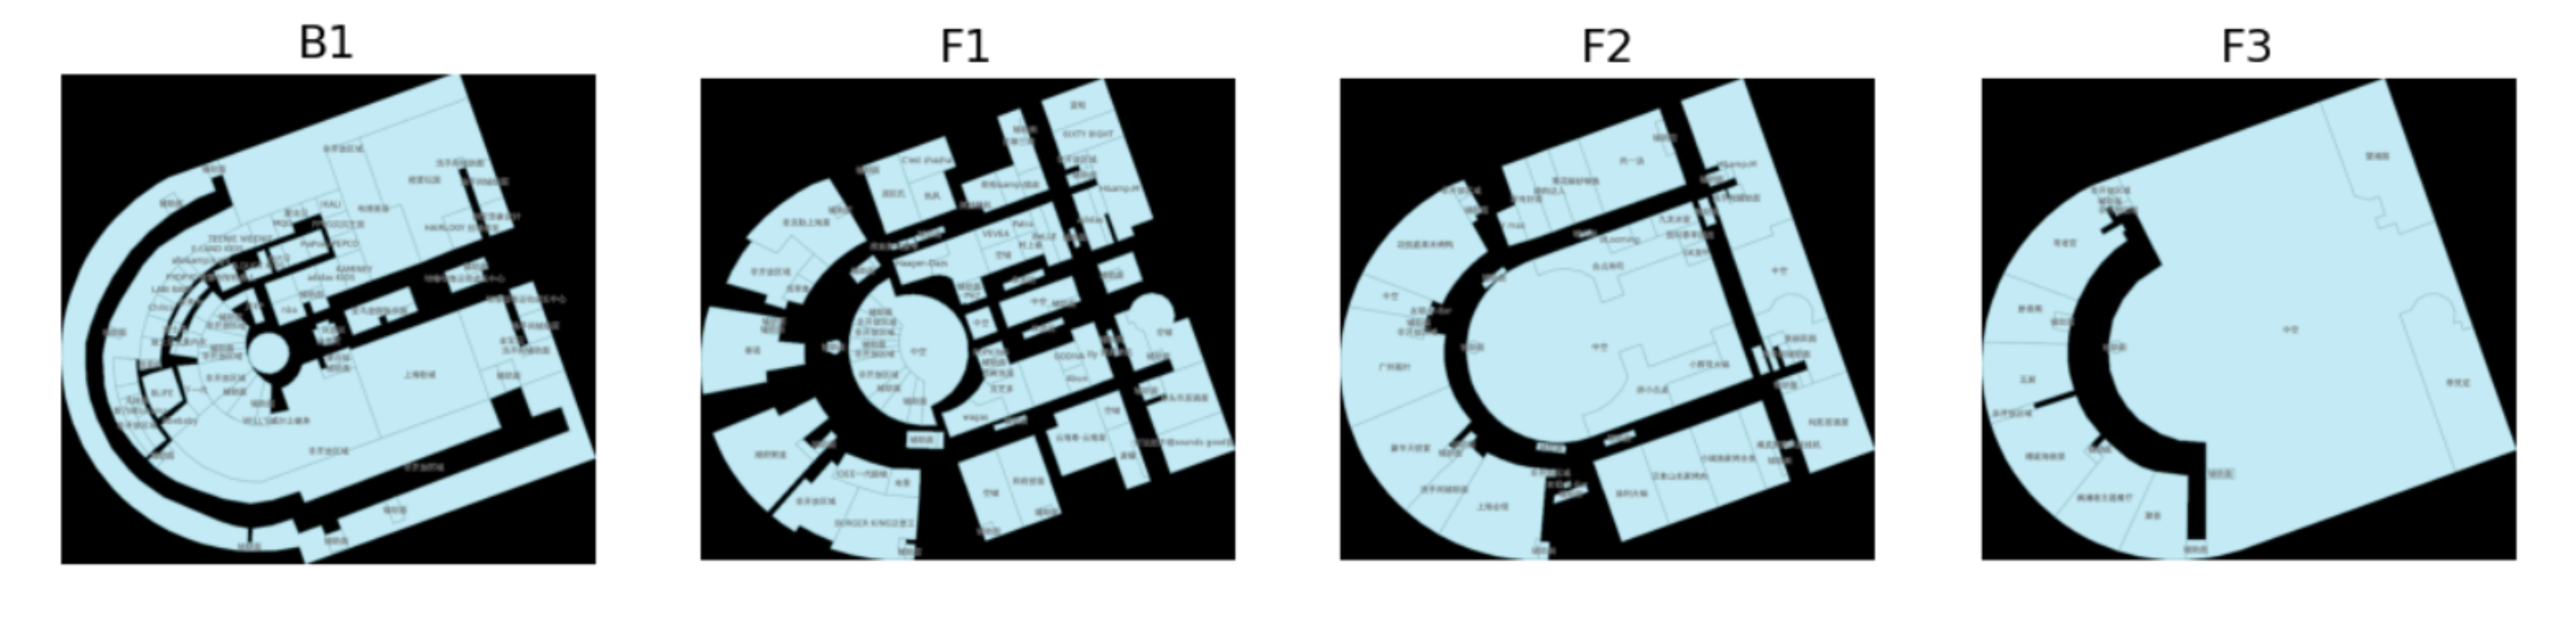
\includegraphics[scale=.31]{Images/ProblemAnalysis/datavisual.png}
    \caption{Depiction of the different floors at a particular site.}
    \label{fig:datavisual}
\end{figure}

Seen on \textbf{\autoref{fig:datavisual}} is an example of a site with its different levels. Level names starting with a B indicates a basement level, where levels starting with F indicates a regular floor. The number indicates the number of levels to the ground from the particular level. The different sites vary a lot in terms of the number of levels.

\begin{figure}[H]
    \centering
    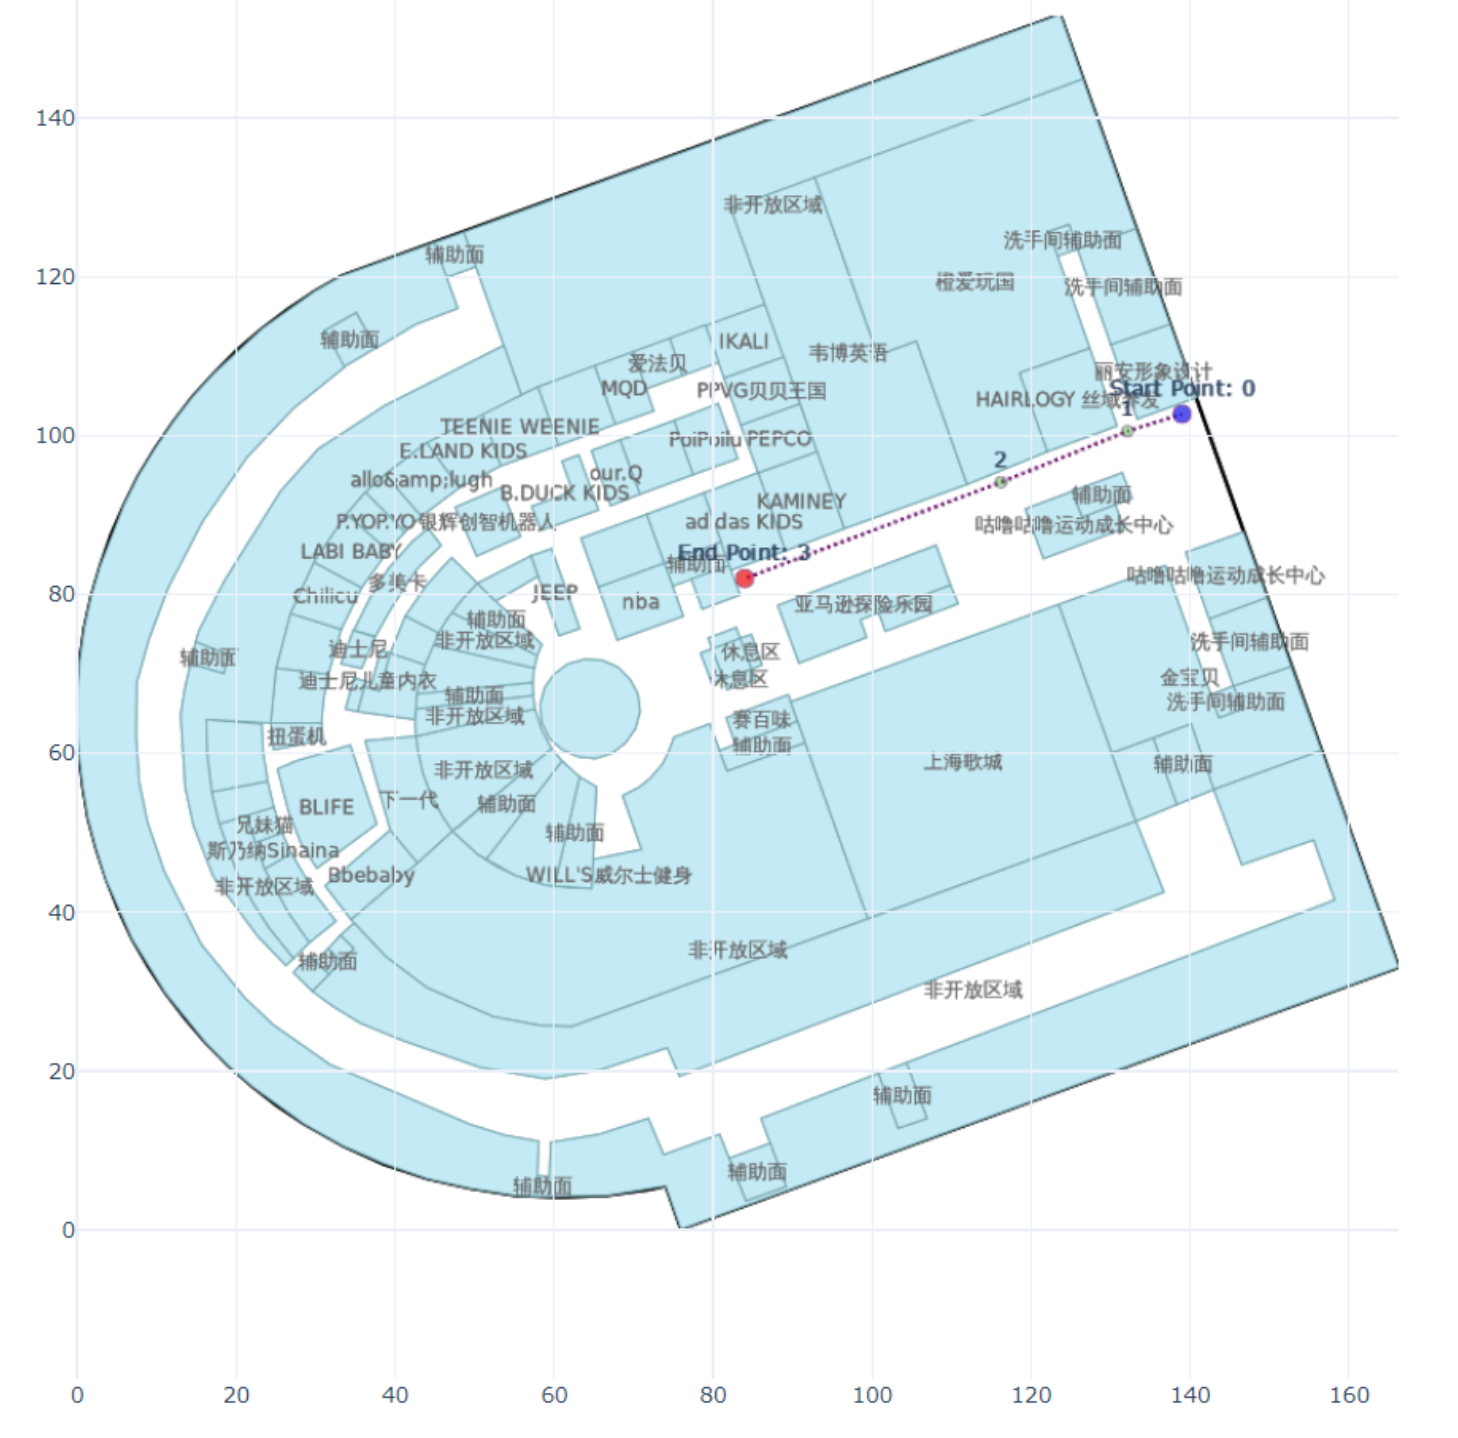
\includegraphics[scale=.37]{Images/ProblemAnalysis/datapath.png}
    \caption{Depiction of a floor with a path from the training data added.}
    \label{fig:datapath}
\end{figure}

It is also possible to view the different paths from the training data on the map of the particular floor. On \textbf{\autoref{fig:datapath}}, we can see the basement floor of the previous figure with one of the paths from the training data. The path on the figure is created from the coordinates of the waypoints (TYPE\_WAYPOINT) in the path file. The blue point is the starting point of the trace and the red point indicates where the path ends. \textbf{\autoref{fig:datapath}} gives an understanding of the distance of a particular path. The different paths vary in size and might cover lesser or larger part of the map. The path given in the figure navigates in a straight line across the room, where other paths can navigate around objects and might trace back to its own starting point.

The training set contains 204 sites. Since we will also have to predict the floor level in addition to the \textit{x} and \textit{y} coordinates, looking into the distribution of floor levels across the training sites could provide insights to whether the class-imbalance problem is present. This problem concerns whether the dataset is well distributed between the classes we want to predict upon. Having a badly distributed dataset could result in the model more often predicting a particular floor level due to a higher occurrence of the aforementioned floor in the dataset, which is not ideal.\cite{Han_Kamber_2012}

\begin{figure}[H]
    \centering
    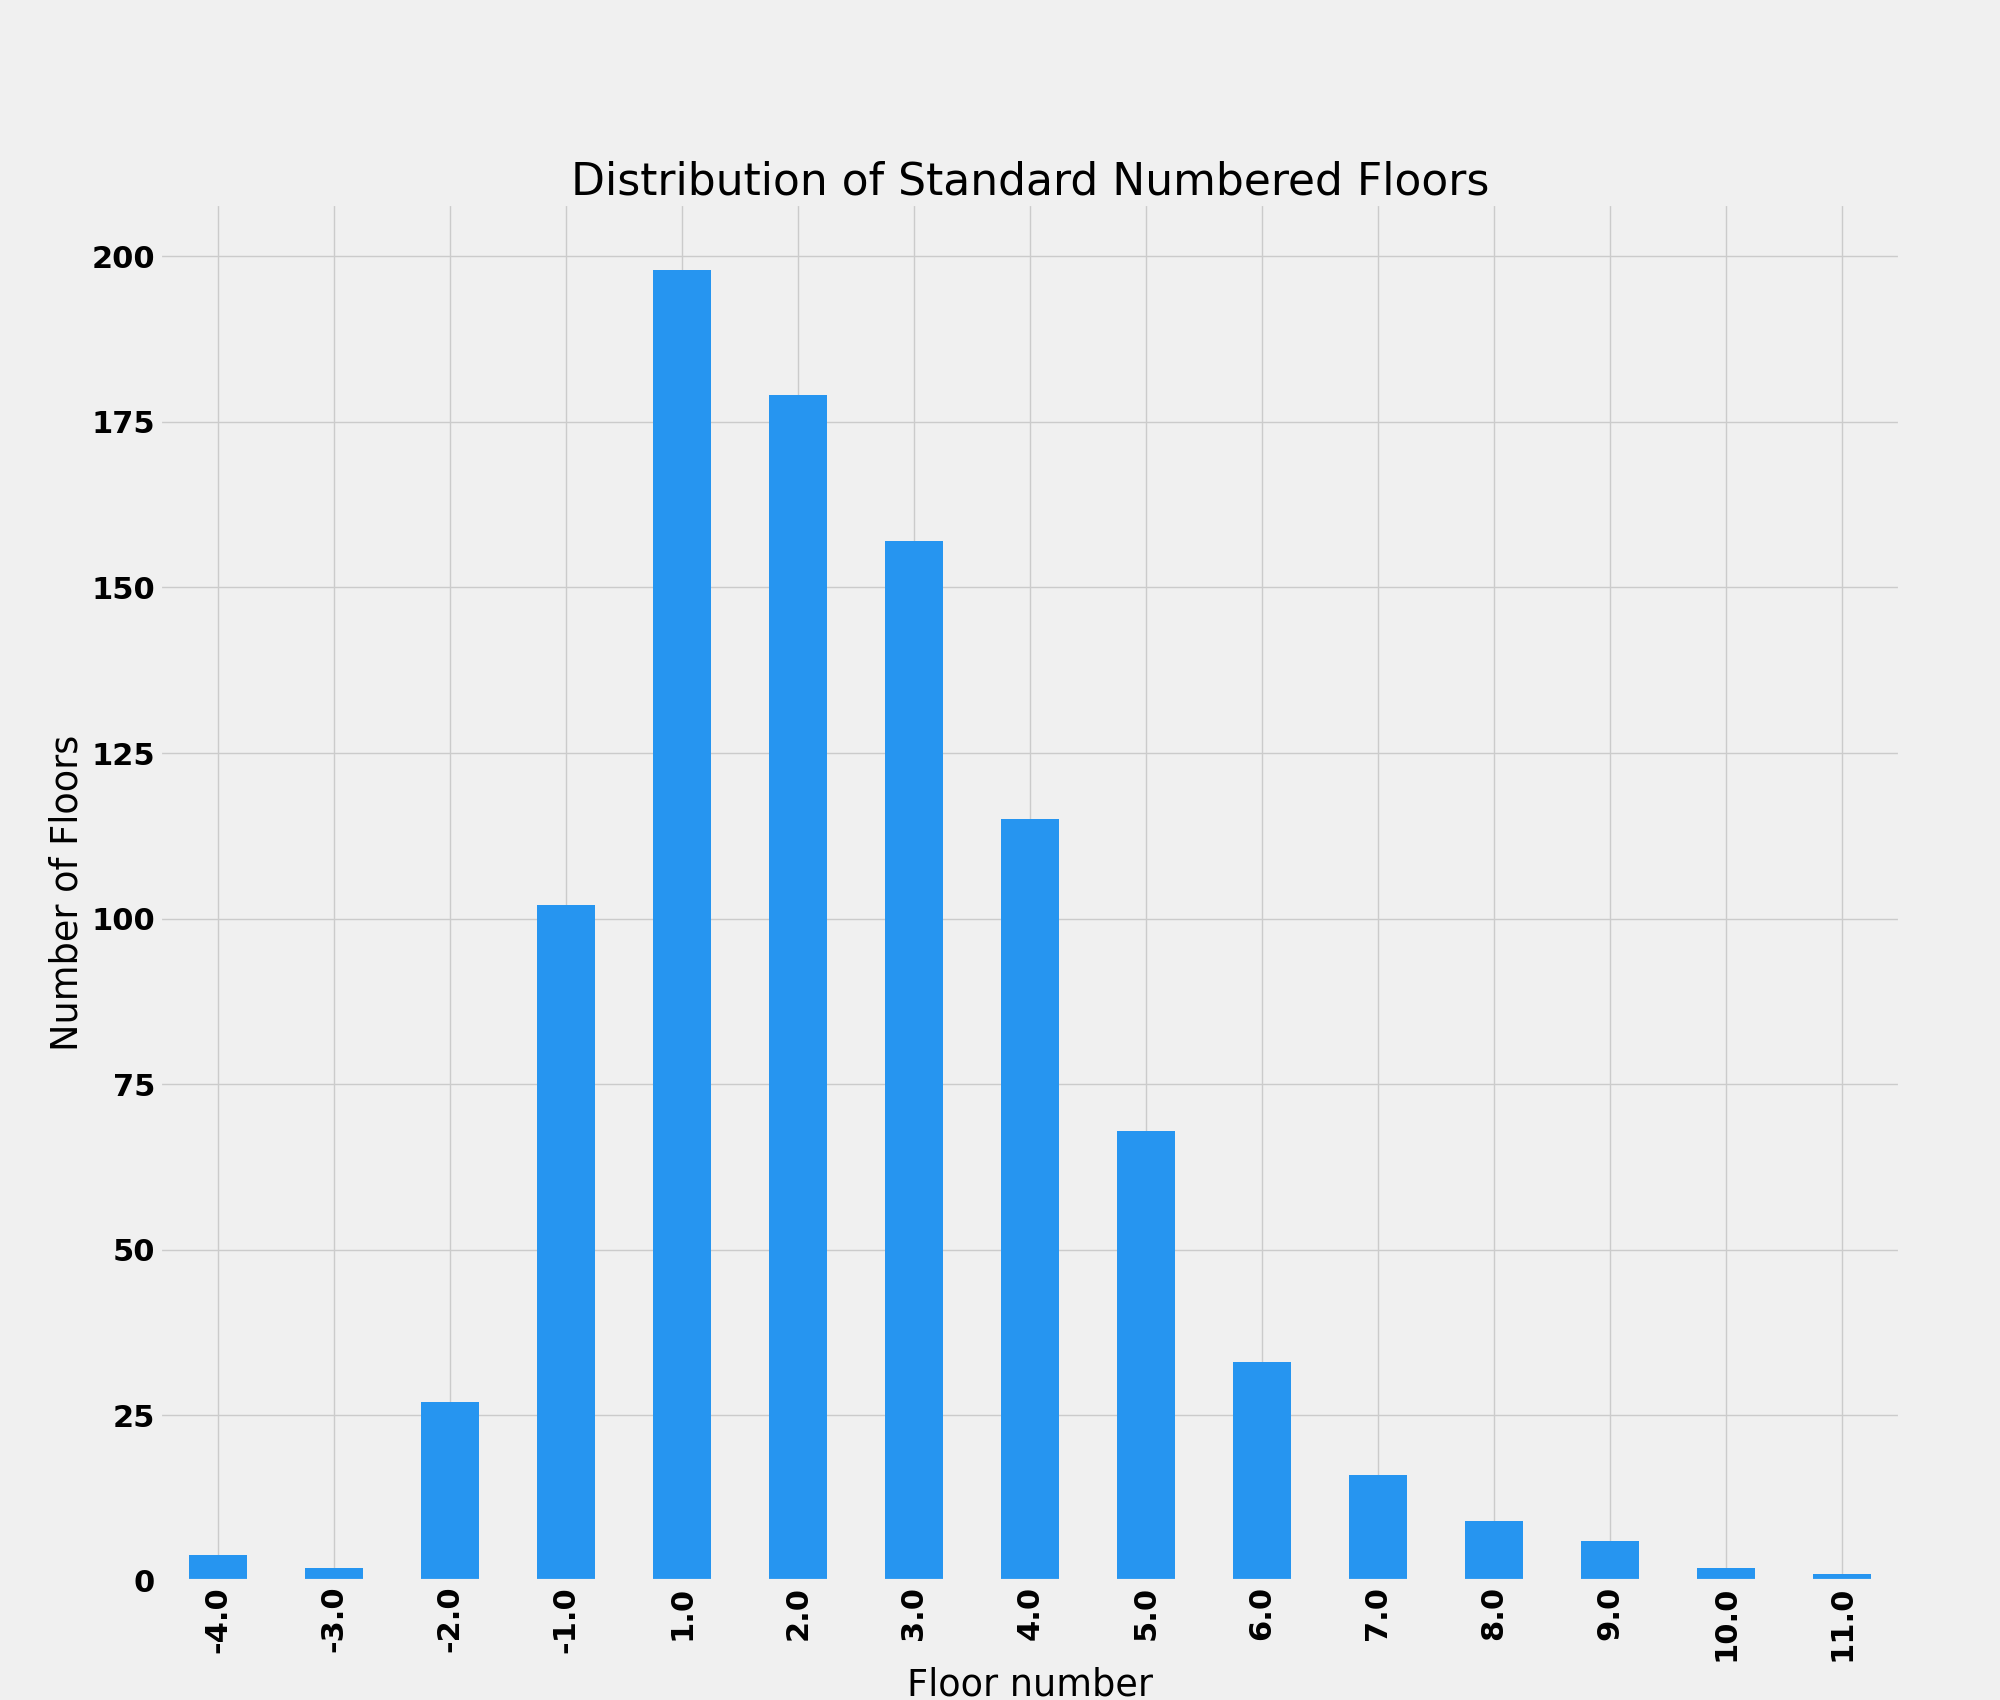
\includegraphics[scale=.15]{Images/ProblemAnalysis/datadistribution1.png}
    \caption{Distribution of standard numbered floors across the data set. X-axis is the floor numbers and y-axis is the number of occurrence of these floors.}
    \label{fig:datadistribution}
\end{figure}

\textbf{\autoref{fig:datadistribution}} displays the number of a particular floor level across the data set. The X-axis denotes the different standard numbered floor levels (positive numbers corresponds to the floors above ground, and the negative numbers corresponds to the basement levels), where the Y-axis describes the number of occurrences of a floor level in the dataset. It is possible from this distribution to see that we possibly have a lot more observations from the floor levels closer to the ground, since they occur more often in the sites in the data set, so this data is also represented in the graph. % Add reason for looking into making an additional distribution on way points per floor.

\begin{figure}[H]
     \centering
     \begin{subfigure}[b]{0.49\textwidth}
         \centering
         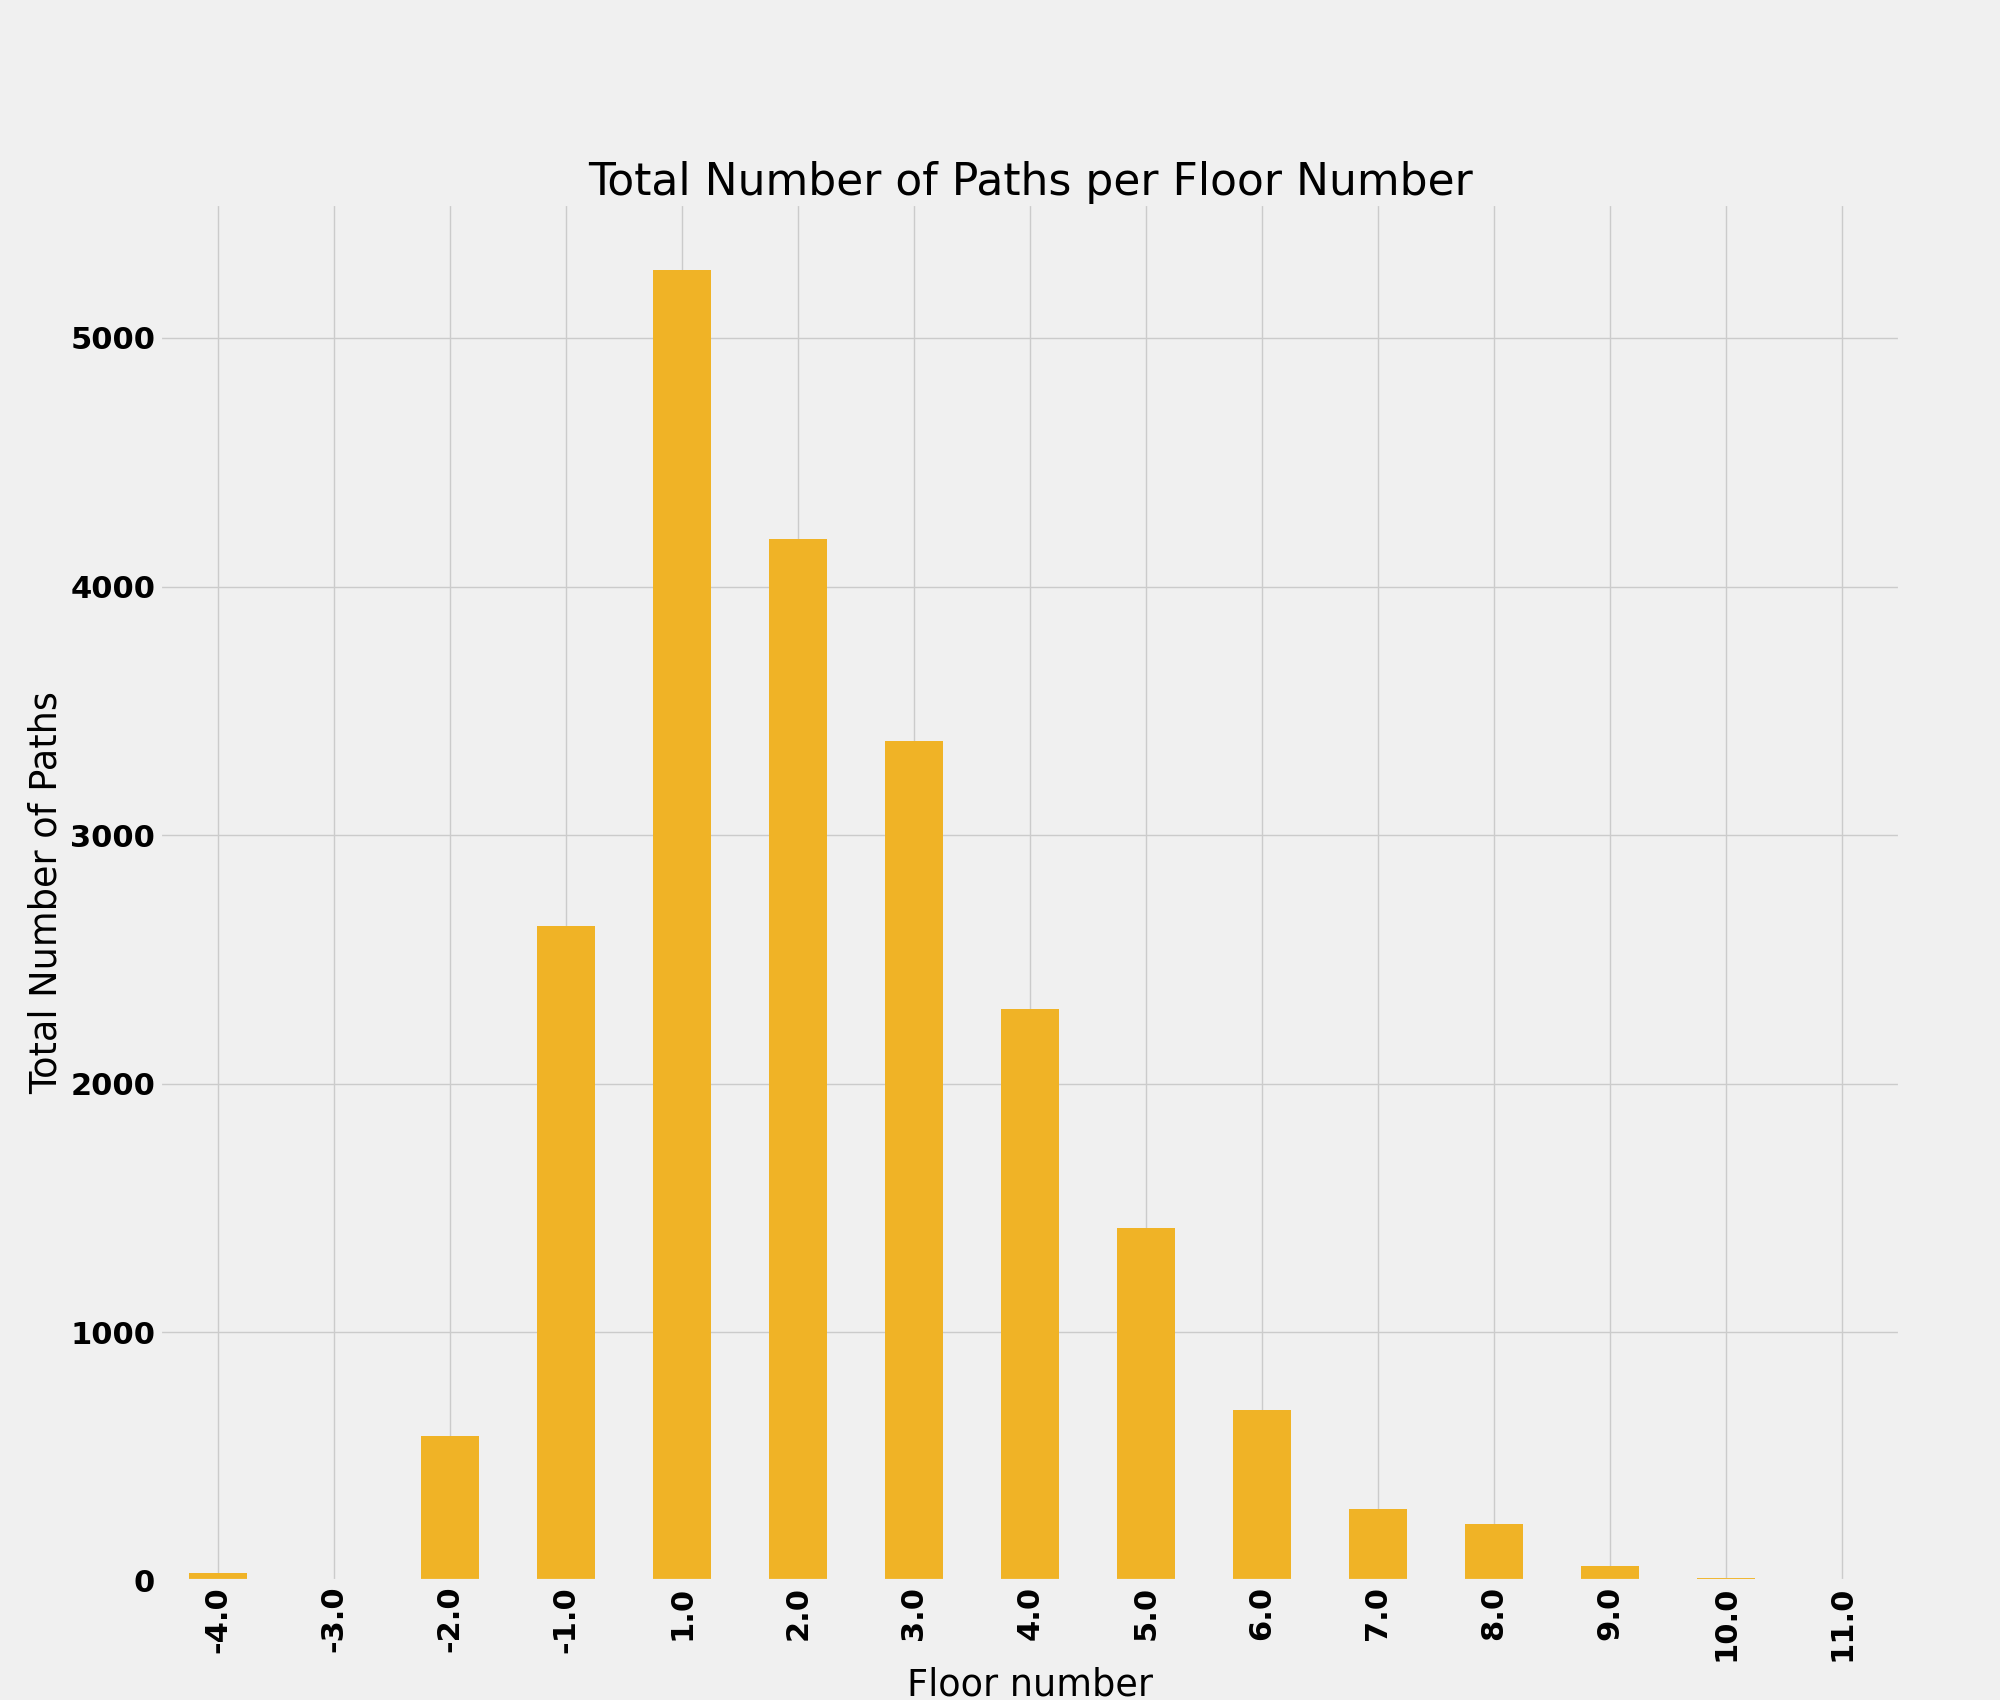
\includegraphics[width=\textwidth]{Images/ProblemAnalysis/datadistribution2.png}
         \caption{Total number of paths per floor number. X-axis is the floor numbers and y-axis is the total numbers of paths on the floors.}
         \label{fig:totalpath}
     \end{subfigure}
     \hfill
     \begin{subfigure}[b]{0.49\textwidth}
         \centering
         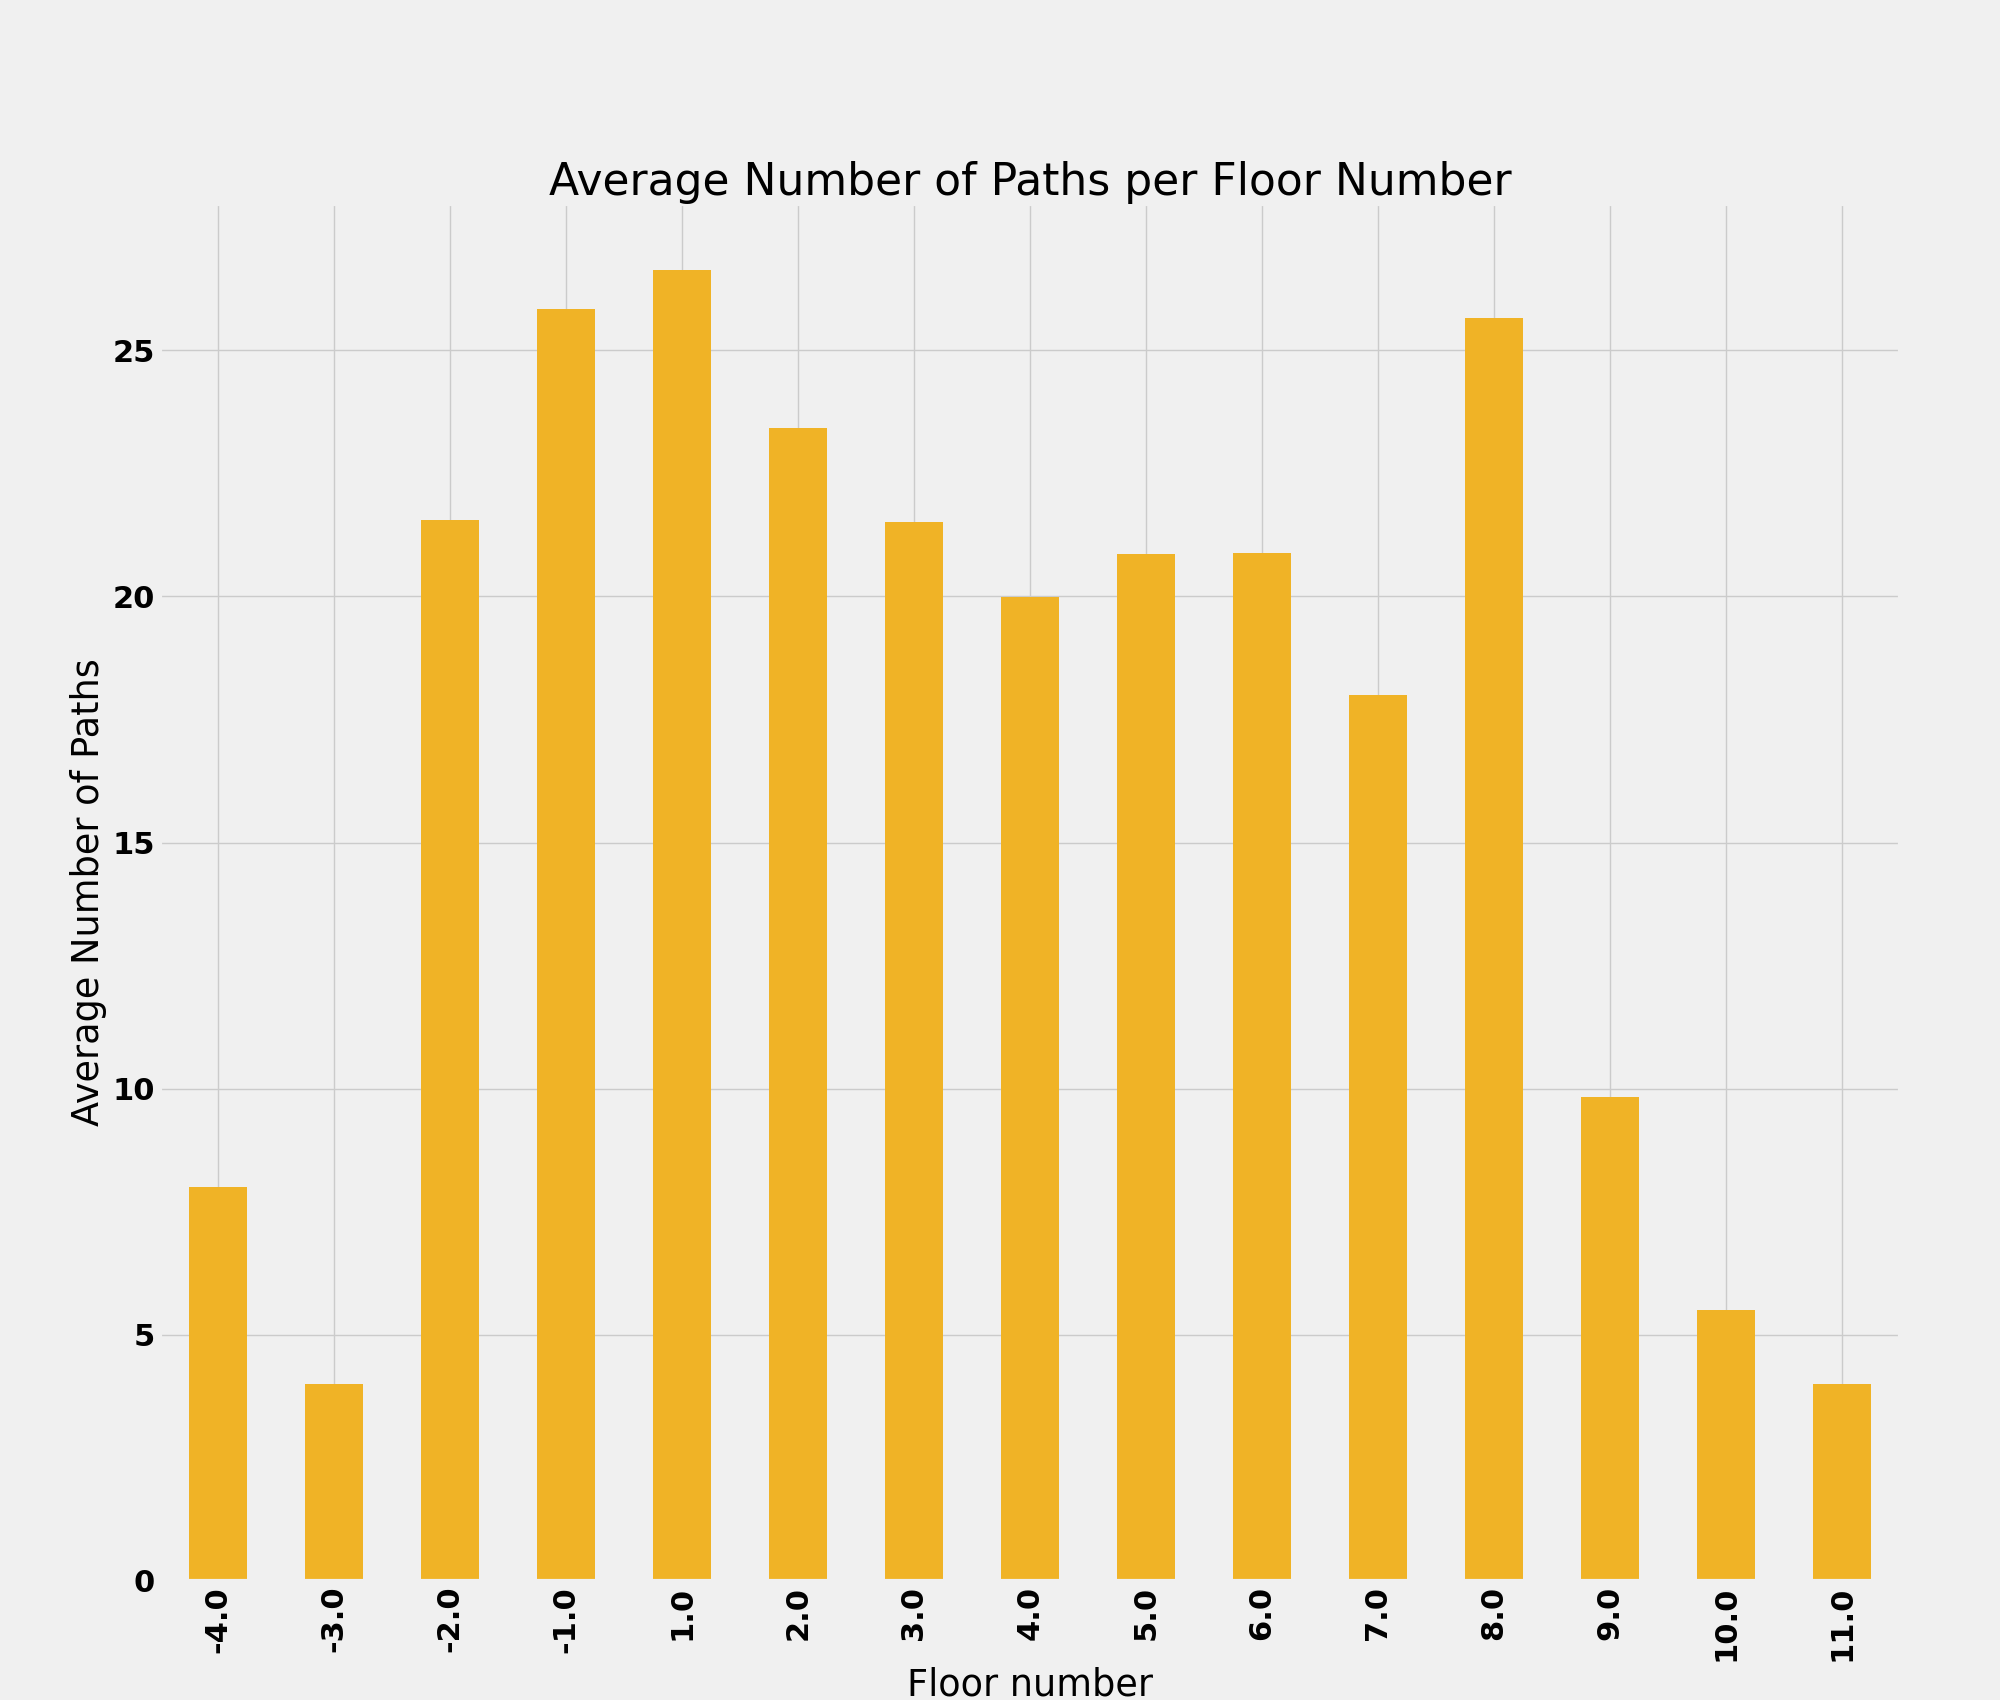
\includegraphics[width=\textwidth]{Images/ProblemAnalysis/datadistribution3.png}
         \caption{Average number of paths per floor. X-axis is the floor numbers and y-axis is the average number of paths on the floor.}
         \label{fig:averagepath}
     \end{subfigure}
        \caption{Distribution of paths in the data set.}
        \label{fig:datadistribution1}
\end{figure}

\textbf{\autoref{fig:datadistribution1}} displays two diagrams of the path distribution in the dataset. In both diagrams, the x-axis denotes floor level and the y-axis describes the number of paths. The first diagram, \textbf{\autoref{fig:totalpath}}, displays the total number of paths across the floor levels, where it is easier to see the difference in occurrences of paths being closer to the ground floor compared to the floors further away. As an example, for the ground floor (F1), we have found 5275 paths across all sites, where for the 10th floor (F11), we only found 4 paths.

Another way to analyse the distribution of paths is to look into the average number of paths for each floor in the dataset. This distribution can be seen on \textbf{\autoref{fig:averagepath}}, which indicates also a large difference between the average number of paths for each floor. A lot of the floors have an average around 20 paths, but floors like the 10th (F11) only have an average of 4 paths.

Alternatively, we can also look into the distribution of waypoints over floors, since the waypoints are the reference locations which will be used to estimate the \textit{x} and \textit{y} coordinates. These distributions can be viewed on \textbf{\autoref{fig:datadistribution2}}.

\begin{figure}[H]
     \centering
     \begin{subfigure}[b]{0.49\textwidth}
         \centering
         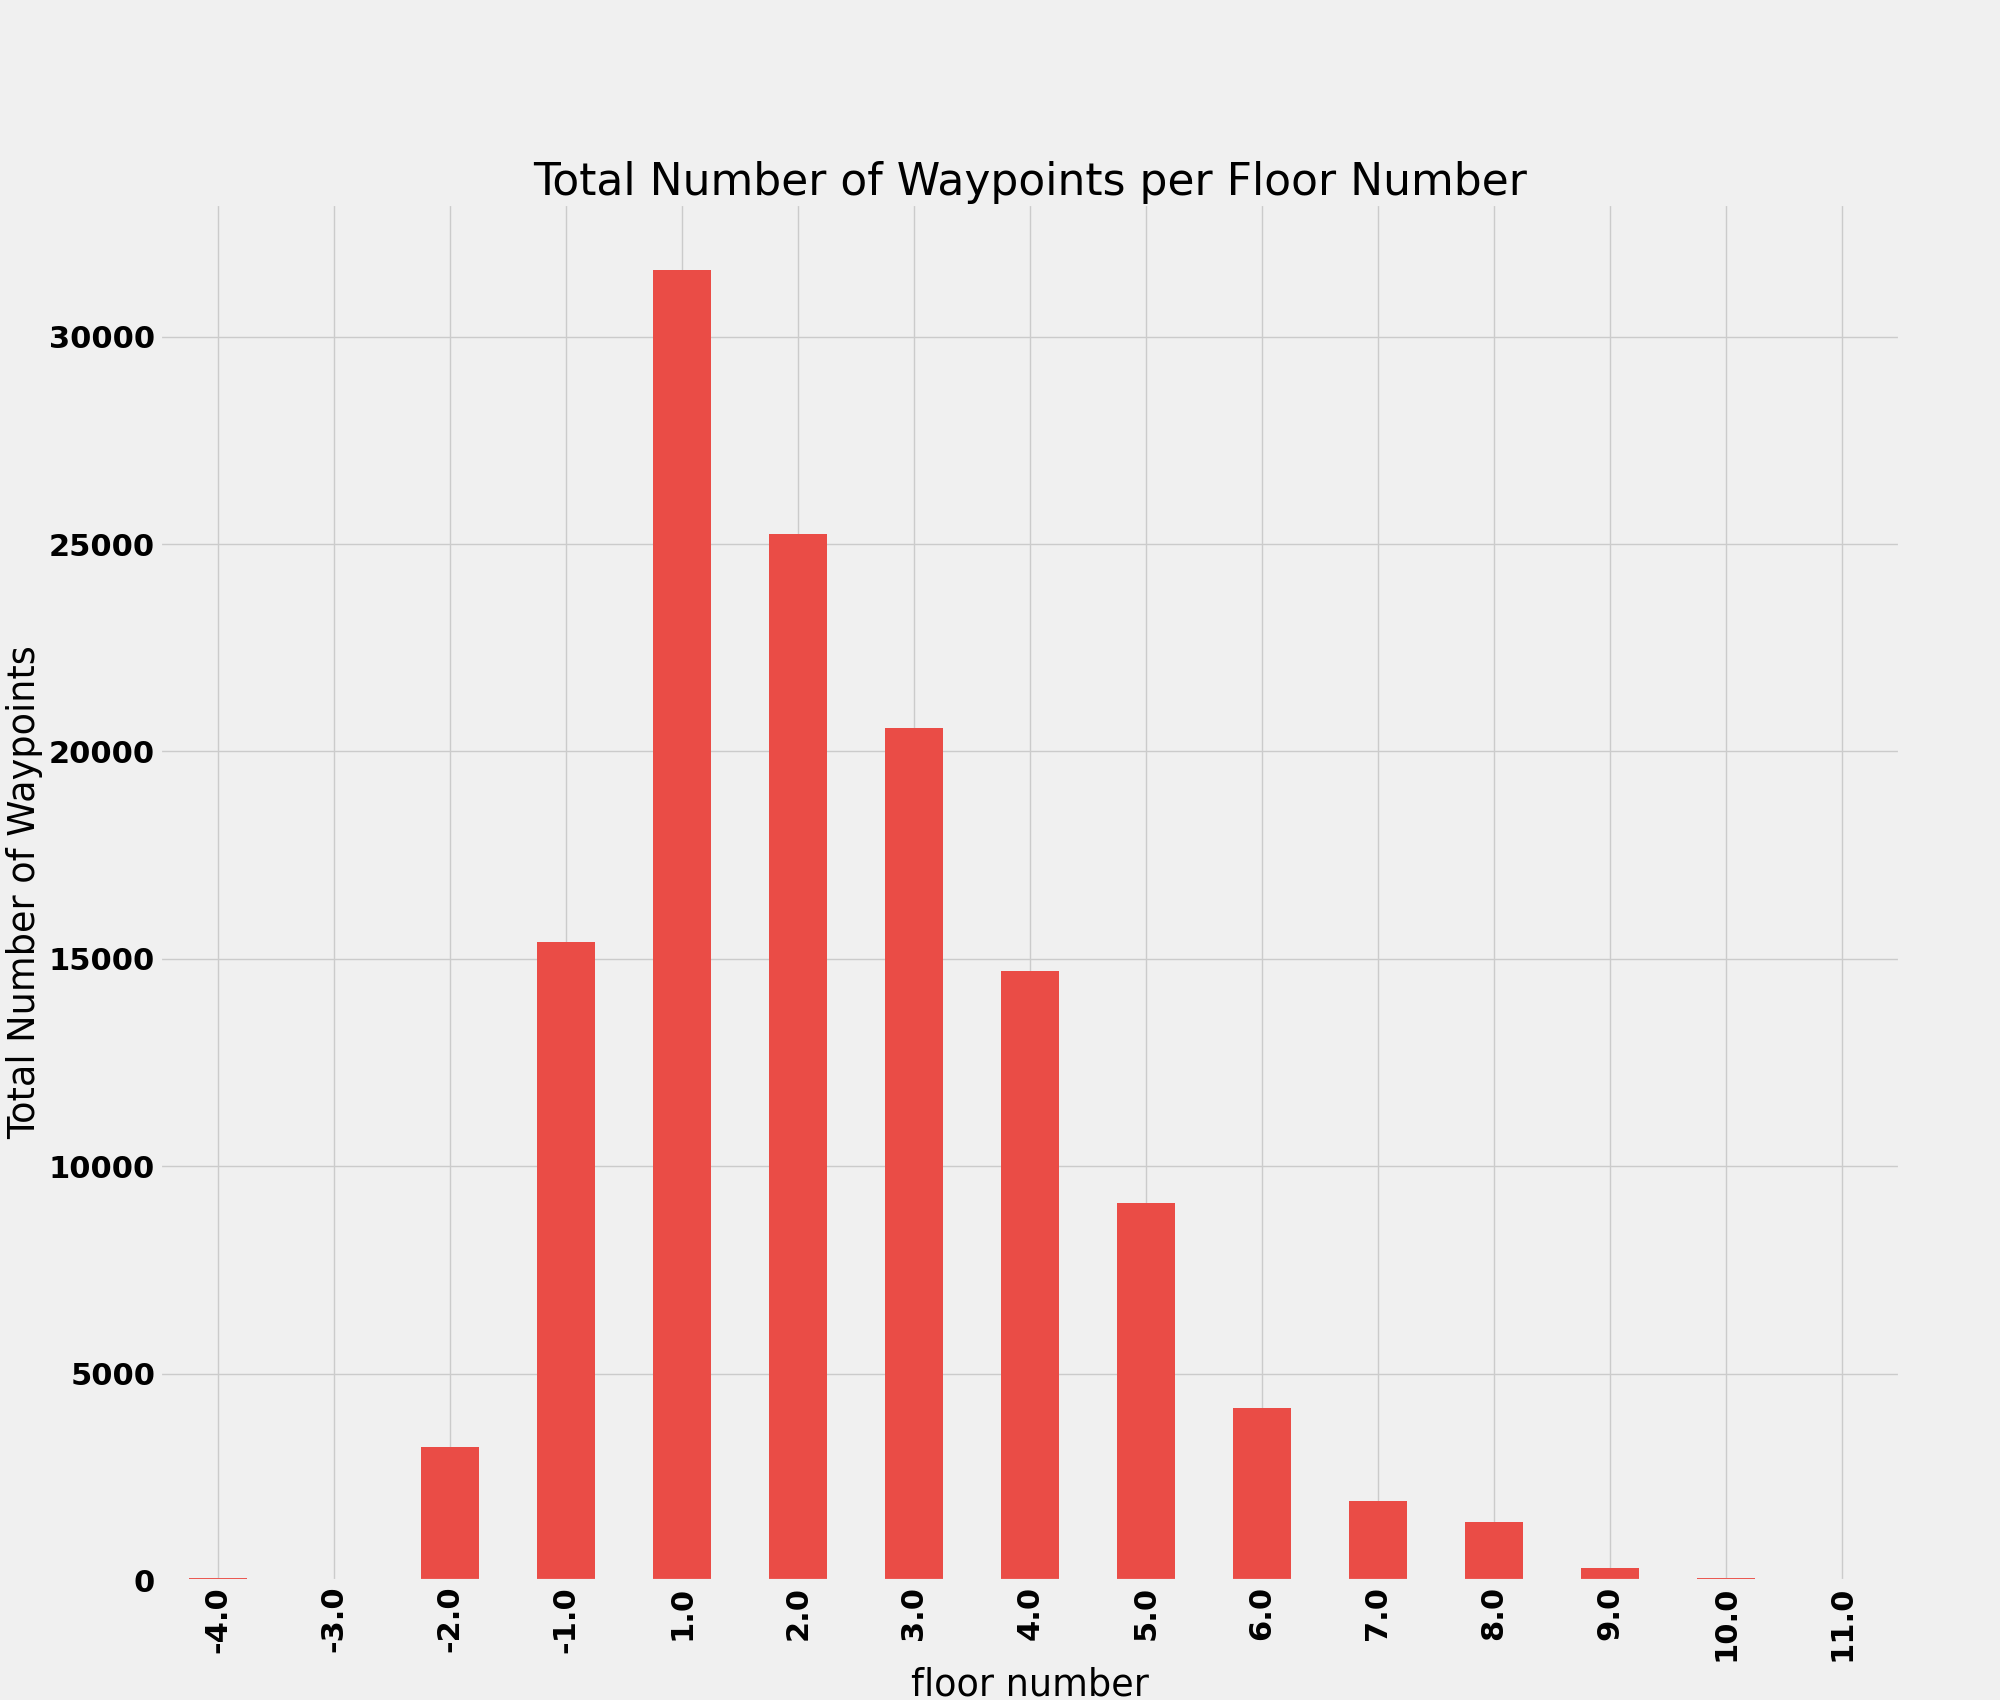
\includegraphics[width=\textwidth]{Images/ProblemAnalysis/datadistribution4.png}
         \caption{Total number of paths per floor number. X-axis is the floor numbers and y-axis is the total numbers of waypoints on the floors.}
         \label{fig:totalwaypoints}
     \end{subfigure}
     \hfill
     \begin{subfigure}[b]{0.49\textwidth}
         \centering
         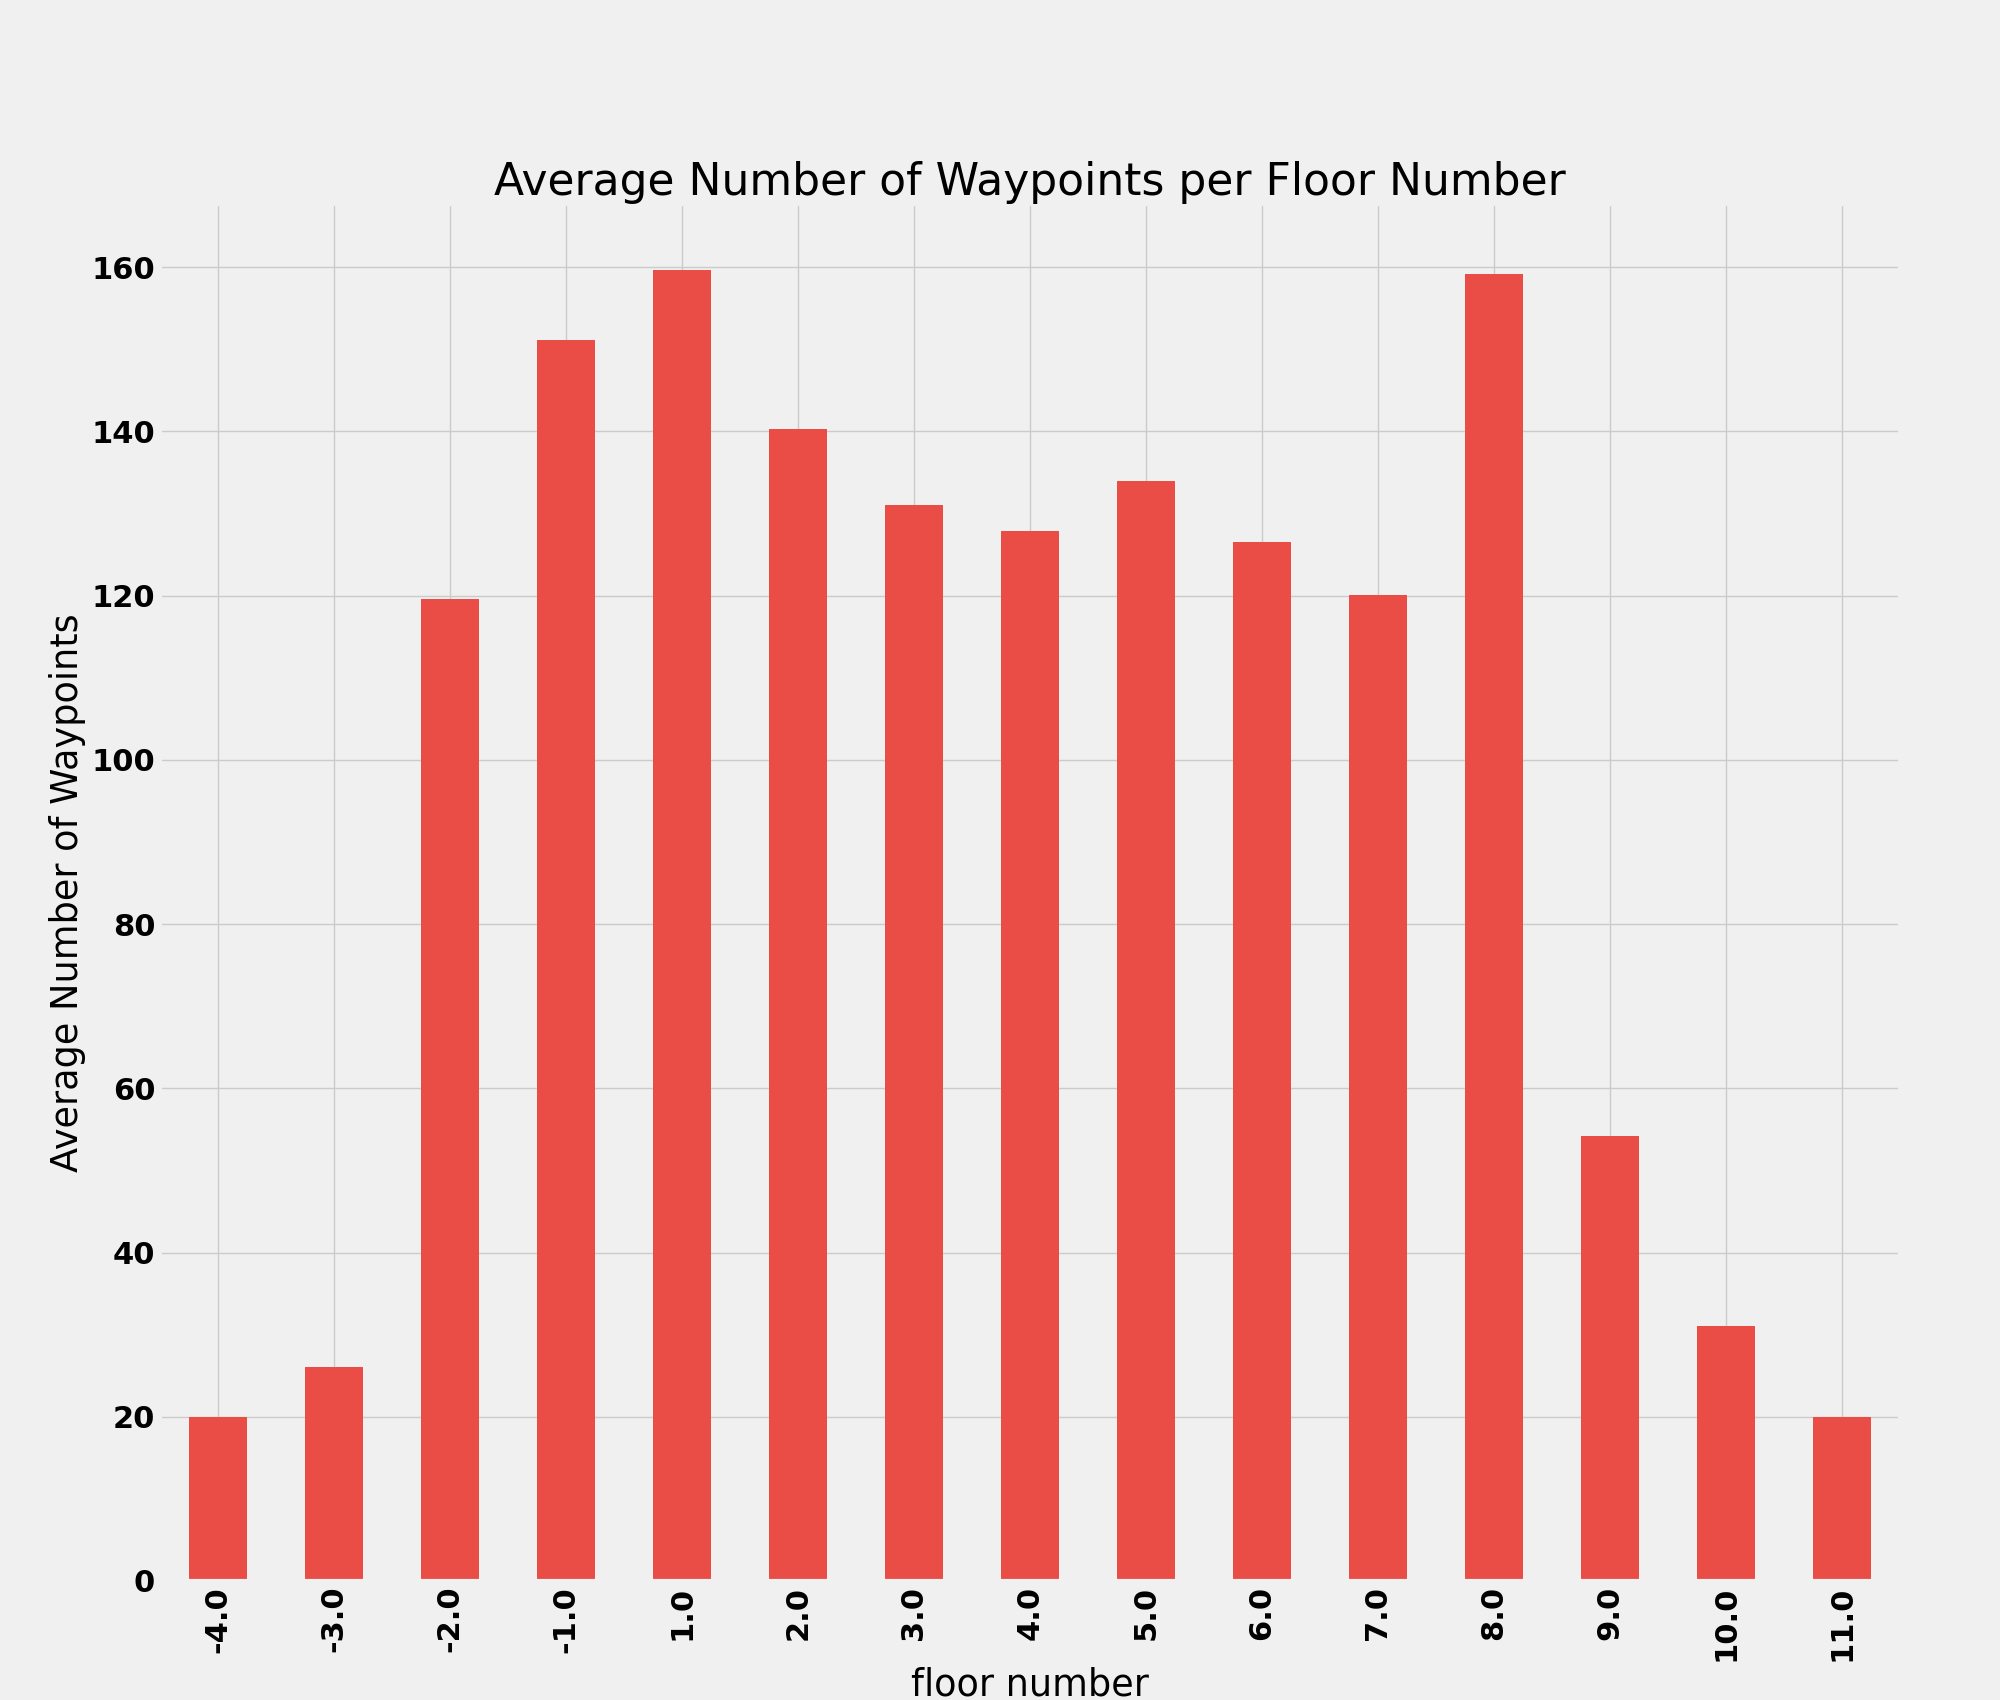
\includegraphics[width=\textwidth]{Images/ProblemAnalysis/datadistribution5.png}
         \caption{Average number of paths per floor. X-axis is the floor numbers and y-axis is the average number of waypoints on the floor.}
         \label{fig:averagewaypoints}
     \end{subfigure}
        \caption{Distribution of waypoints in the data set.}
        \label{fig:datadistribution2}
\end{figure}

\textbf{\autoref{fig:totalwaypoints}} displays the number of waypoints for each floor. The distribution is looking quite similar to \textbf{\autoref{fig:totalpath}}, which could indicate a similar amount of waypoints for each path. To ensure this hypothesis we decided to look into the average number of waypoints per floor as seen on \textbf{\autoref{fig:averagewaypoints}}. This yielded a bit different distribution compared to \textbf{\autoref{fig:averagepath}}, where we can see that the 4th basement level (-4 or B4) has a quite lower average in waypoints per floor than paths per floor, which indicates having more paths but with lesser waypoints in them.

%The test set contains 626 paths to predict upon.


% Måske tjekke distribution på antallet af entries for de forskellige floors.
% boxplot over number of levels (lowest/highest)
%Cleaning the data based on the previous section - maybe even the distribution



%\subsection{Data Cleaning}





\section{Existing Positioning Methods} \label{sec:existingpositioningmethods}
In this section, we will consider positioning algorithms, which can be used to estimate the location. The positioning algorithms can be divided into three types, namely geometry-based algorithms, positioning algorithms using scene analysis, and positioning algorithms using inertial measurements. Each of the algorithm types have their own weaknesses and strengths. Therefore, combining more than one algorithm could potentially lead to a better estimate of the location. 

\subsection{Scene Analysis}
\label{sec:scene_analysis}
Algorithms which perform scene analysis work by first constructing fingerprints for a scene, then estimate the location by matching online measurements against the locations' fingerprints. This type of algorithms is also called location fingerprinting. Location fingerprinting consists of two phases, namely the offline phase and online phase. In the training phase or offline phase, the data, typically radio frequency data, is collected at access points for different known indoor positions, and a fingerprint is constructed for known indoor positions. During the online phase, the real time position is estimated by pattern matching the measured data with the fingerprints of the locations from the offline phase.\cite{IPS01} The following machine learning algorithms can perform location fingerprinting.

\subsubsection{LightGBM}
As LightGBM is a widely used algorithm by other competition participants at Kaggle, we will also be investigating this algorithm.
LightGBM is a variation of the \gls{gbdt} algorithm. \gls{gbdt} is an ensemble model of decision trees, which are trained in sequence. In each iteration, the \gls{gbdt} learns the parameters of the decision trees. A decision tree is a tree which consists of internal and leaf nodes. The internal nodes have a condition based on the observations or the input and contain two children nodes. One of the children nodes will be labeled true while the other is labeled false. Each leaf node is labeled with a class, and the classification will be the labeled class at the leaf node depending on which leaf node is reached within the tree\cite{AIBook}.
The LightGBM significantly outperforms other \gls{gbdt} algorithms like XGBoost and Stochastic Gradient Boosting in terms of computational speed and memory consumption, which is ideal for our case as the model should be made available on a mobile application/service. \cite{lightgbm} LightGBM is not widely used in \gls{ips} when relating to research in \gls{ips}. In the Kaggle competition, \cite{lgbmKaggle01} uses LightGBM and Wi-Fi \gls{rssi} measurements to achieve a public score of 8.34 meter based on the evaluation metric defined in \textbf{\autoref{sec:kaggleComp}}. The aforementioned LightGBM implementation achieves the lowest \textit{mean positioning error} for the LightGBM implementations at Kaggle.

\subsubsection{Artificial Neural Network}
Neural Networks are inspired by the neurons in the brain. The networks consist of neurons or units organised into layers. The typical neural network architecture is the \gls{ann}. This type of network consists of an input layer, an output layer, and a number of hidden layers\cite{AIBook}. 

The use of \gls{ann} in \gls{ips} has among other been investigated by \cite{ANN01}. The \gls{ann} model proposed by the paper consists of an input layer with four neurons, an output layer with two neurons, and four hidden layers. The indoor positioning system proposed by the paper only considers Wi-Fi \gls{rssi} data. As input to the model, it uses normalised Wi-Fi \gls{rssi} measurements from each of the access points. The environment in the paper consists of four access points and thus results in four input neurons. The output of the model will be the \textit{x} and \textit{y} coordinates. Furthermore, the amount of hidden layers for the model should depend on the number of input and output neurons. The performance of the model is evaluated through precision in the form of the \textit{position error}, and accuracy in the form of \textit{Mean Position Error}. The result of the ANN is that the ANN can achieve a error of less than 1 meter for 30\% of the instances, 10\% of the instances has an error more than 2 meters, and 60 \% of the instances has an error of 1-2 meter. 

\cite{ANN02} also investigates the feasibility of \gls{ann} in \gls{ips}. This method also uses Wi-Fi \gls{rssi} measurements as input data. Here, the results are summarised by the \textit{mean position error} and the training time for the \gls{ann}. The results are measured for two scenarios, one complex environment with increased interference and another environment with less interference. The \textit{mean position error} is around 0.21 meter for all configuration of \gls{ann} in the complex environment and 0.1 meter for the simple environment. 

The main challenge with \gls{ann} is to find the balance between computation time and performance as it is possible to achieve greater performance with deeper networks but this would also result in more computation time and therefore might not be ideal to implement in a mobile device. However, model compression techniques can be used to compress a deep network model.

\subsubsection{kNN}
The \textit{k}-Nearest Neighbors algorithm works by first finding \textit{k} nearest neighbors through a distance metric. After finding the \textit{k} nearest neighbor, the classification or prediction will be the majority of the neighbors. In a position estimation setting, instead of considering the majority of the neighbors, an average of the \textit{k} nearest neighbors is calculated. This average would then be the location estimate. The most commonly used distance metric in positioning is the Euclidean distance. \cite{IPS01} In the IPS context, a Weighted \textit{k}-Nearest Neighbors algorithm (WKNN) has been investigated by \cite{wknn}. In the WKNN, the \textit{k} nearest neighbors are first weighted according to some weights before averaging them. In this paper, the Manhattan distance achieves better results compared to the Euclidean distance. WKNN achieved an error of 1.07 meter for 80\% of the errors, and approximately 2 meter for all of the errors. This algorithm can also be used in real-time application.
%https://link.springer.com/article/10.1007/s11277-017-4295-z
%https://ieeexplore.ieee.org/stamp/stamp.jsp?tp=&arnumber=8054235

\subsubsection{Hidden Markov Model}
In the \gls{hmm}, the idea is to consider a series of measurements instead of a single signal measurements, which greatly improved the location estimation accuracy. This series of measurements makes it possible to keep track of a device's location over time. \gls{hmm} consists of two types of states, namely the observable states and hidden states. The observable states are denoted by the shaded circles in \textbf{\autoref{fig:hmm}}, while the hidden states are denoted by the shaded circles. \gls{hmm} assumes that hidden states only depends on the observable states. In the \gls{ips} context, the observable states will be the signal measurements like Wi-Fi \gls{rssi} while the hidden states will be the locations. \gls{hmm} has a transition probability distribution, and an emission probability distribution. The transition probabilities models the state at time $t$ based on time $t-1$ meaning that the history of device' locations are captured in the transition probability. The emission probabilities models the probability of a particular observation being made at a state.\cite{hmmOverview}

\begin{figure}[h]
    \centering
    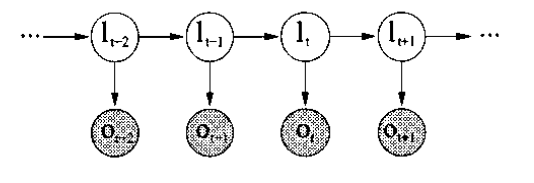
\includegraphics[scale=1.6]{Images/ProblemAnalysis/hmm_pe.PNG}
    \caption{Graphical representation of \gls{hmm} in the \gls{ips} context. The white nodes are the locations and hidden states of the model. The shaded nodes are the signal measurements, and are the observable states of the \gls{hmm} \cite{hmmOverview}}
    \label{fig:hmm}
\end{figure}

A \gls{hmm}-based approach is investigated by \cite{hmm01}. The approach uses Wi-Fi \gls{rssi} measurements as the input or observable states. In this approach, the transition probabilities are modelled by displacement ranging, where step counting and stride length are considered. Furthermore, to reduce the computation overhead when using this approach \textit{k}-nearest is used to reduce the amount of location candidates considered. This approach achieves a \textit{mean position error} of less than 1 meter for 50\% of the instances, while for 80\% of the instances the error is 2.5 meters, and for all of the data instances the \textit{mean positioning error} is at 5 meters.

% \begin{longtable}{ p{.25\textwidth}  p{.7\textwidth}}
% \textbf{Tree Based Learning} & Tree based learning employs decision tree(s) or classification tree(s) for classification. A decision tree is a tree which consists of internal and leaf nodes. The internal nodes has a condition based on the observations or the input and contains two children nodes. One of the children nodes will be labeled true while the other is labeled false. Each leaf node is labeled with a class, and the classification will be the labeled class at the leaf node depending on which leaf node is reached within the tree.\cite{AIBook}
% \\\\
% \textbf{Neural Network} & Neural Networks are inspired by the neurons in the brain. The networks consist of neurons or units organised into layers. There are many different types of neural networks, where the typical network architecture is feed-forward neural networks. This type of network consist of an input layer, an output layer, and a number of hidden layers.\cite{AIBook} 
% \\\\
% \textbf{kNN} & The \textit{k}-Nearest Neighbors algorithm works by first finding \textit{k} nearest neighbors through a distance metric. After finding the \textit{k} nearest neighbor, the classification or prediction will be the majority of the neighbors. In position estimation setting, instead of considering the majority of the neighbors, an average of the \textit{k} nearest neighbors is calculated. This average would then be the location estimate. The most commonly used distance metric in positioning is the Euclidean distance. \cite{IPS01}
% \\\\
% \textbf{Probabilistic Model} & The probabilistic model are based on Bayes' rule, and models the problem in terms of probabilities. One probabilistic method is to, given a measured signal and a number of location candidates, model the probability of each of the location candidates conditionally dependent on the measured signal. The location candidate with the highest probability would then be the location estimate.\cite{IPS02}. Other probabilistic models could also be useful in position estimation such as the Hidden Markov Model, where we in addition to the measured signal also consider the previously measured signals when estimating a position.
% \\%\\
% %\caption{presents the main recommender system types.}
% \label{table:fingerprinting}
% \end{longtable}

\subsection{Geometry-Based Methods}
In this section, we will describe three different techniques to estimate a position of an object geometrically.

\subsubsection{Triangulation} \label{sec:triangulation}
Triangulation is described in \cite{Triangulation}. Triangulation is based on using angles of known points in space. Among the triangulation based methods, four popular types exist. The four types use different types of data, which are \gls{toa}, \gls{tdoa}, \gls{aoa}, or signal strength (\gls{rssi}).

\begin{figure}[H]
    \centering
    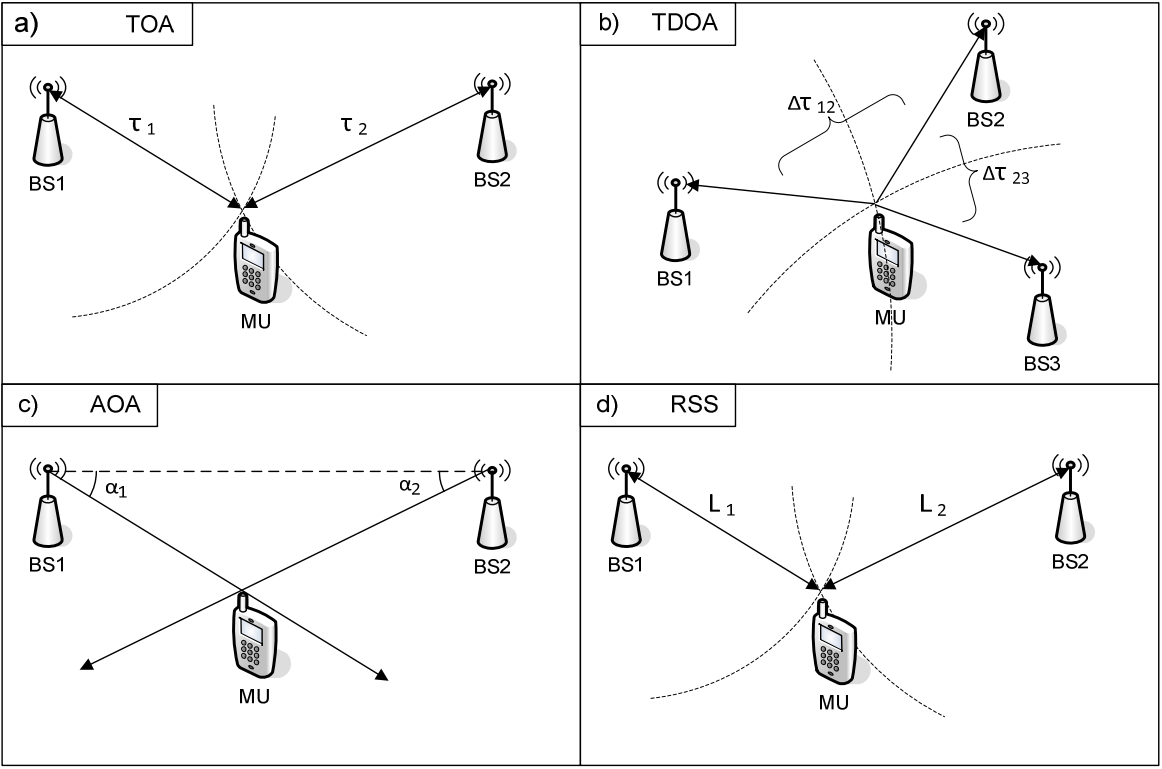
\includegraphics[scale=0.9939]{Images/ProblemAnalysis/triangulation.PNG}
    \caption{Overview of the four popular triangulation methods.\cite{triangulation01}}
    \label{fig:triangulation}
\end{figure}

We will now elaborate on the popular methods described in \textbf{\autoref{fig:triangulation}}. In the method using \gls{toa}, the time to transmit a signal from a base station to a mobile device is recorded and used to calculate the distance inbetween. This, however, requires precise time synchronisation between all devices which could be cumbersome. In the methods using the \gls{tdoa}, the mobile device transmits positioning signals to nearby measuring units, and the \gls{tdoa} is estimated and used for the positioning. In the methods utilising \gls{aoa}, the basic idea is to use goniometry to estimate the position. The base stations contain antennas to measure the angle of the incoming signals from the mobile device. This information is then used to estimate the position of the device.\cite{triangulation01}

Triangulation does not seem to be accurate in the indoor positioning setting as several paper find other methods more accurate compared to it \cite{triangulation02}\cite{triangulation03trilat}. However, it might be possible to combine it with other methods, like location fingerprinting, which could result in better performance\cite{triangulation4}. AS it does not perform well on its own, we will not be working with this method.

\subsubsection{Trilateration} \label{sec:trilateration} 
Trilateration is described in \cite{Triangulation}. In trilateration, the basic idea is to compute the point of intersection between the three circles defined by the beacons. The point of intersection is the position of the mobile device and can be calculated by using the mathematical definitions of the circles created by the signals transmitted from the beacons. This is illustrated in \textbf{\autoref{fig:trilateration}}, where $a$, $b$ and $c$ are the beacons, $m$ is the position of the device to be located, and $l$ values, with respect to each beacon, are the radii of each circle.
%In trilateration, the position of an object is calculated by solving three equations defining the circles. This is illustrated in \textbf{\autoref{fig:trilateration}}.
%By letting the beacons be denoted as $a$, $b$ and $c$, and the object to locate $m$, we can solve the the three equations to compute the location of $m$, where $l$ is the radius of each circle.

\begin{figure}[H]
    \centering
    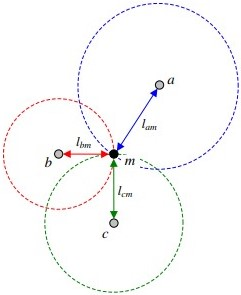
\includegraphics[scale=0.8]{Images/ProblemAnalysis/trilateration.jpg}
    \caption{Illustration of locating an object using three beacons with the use of trilateration\cite{Triangulation}.}
    \label{fig:trilateration}
\end{figure}

In the indoor positioning context, trilateration does not seem as the ideal solution\cite{trilateration02}. One of the key findings in \cite{trilateration02} is that trilateration is infeasible in \gls{ips}. Some papers also use trilateration in comparison to other methods to illustrate that the other methods achieve better performance \cite{triangulation03trilat, trilateration01}. Due to the aforementioned reasons, we will not be implementing trilateration for our indoor localisation method.


\subsubsection{Centroid}
The centroid localisation algorithms are described in \cite{5759777}. Centroid is, like triangulation and trilateration, based on beacons and the locations of the beacons. The goal is to provide a location estimate of an object given a vector of \gls{rss} values. There exists two algorithms to locate an object: a range-based, which uses several distance to beacon estimations obtained from \gls{rss} measurements, and a range-free, which determines a location without distance estimations. These two algorithms are identified as \gls{wcl}\cite{5759777} and \gls{rewl}\cite{5759777}, respectively.

\gls{wcl} approximates the location of an object by calculating the centroid of the coordinates of the beacons that are in range. Using this algorithm, the distance from the object to each of the beacons within range is taken into account.
In the estimation of the position of an object using \gls{rewl}, \gls{rewl} favors the beacons transmitting with higher \gls{rss} values, since those are likely to be closer to the object.

\cite{7536951} implemented an indoor localization system using the centroid approach using WCL. The system achieved an accuracy of around 2 meters.

This method requires additional information, namely the location of the beacons. Therefore, to implement a localisation system using the centroid method requires a way to provide these beacon locations for the position estimation. As this is not widely available in the mobile context, we will not be using this method.

\subsection{IMU positioning} \label{sec:IMUPositioning}
Location estimation with the use of IMU is described in \cite{IMUPositioning}. As mentioned in \textbf{\autoref{sec:actuator_sensor}}, IMU consists of an accelerometer, a gyroscope and a magnetometer, and makes use of these to compute a position. Using IMU positioning, one can compute a position by the displacement of an initial position. This is also the disadvantage of IMU positioning, namely that an initial position is required.

To compute a position using IMU positioning, one starts by using the Euler method to compute the velocity of the moving object given data from the accelerometer, and then uses the the Euler method to compute the displacement from an initial position. Combining the results of these two computations along the current accelerator reading, the total displacement can be computed.

As just mentioned, the only requirements to implement indoor positioning using IMU are an initial position and that the sensors that make up an IMU are integrated within the mobile device. Therefore, we will experiment with indoor positioning using the Euler method and \gls{pdr}, which is mentioned in the following section.

\subsubsection{\acrlong{pdr}}\label{sec:pdr}
The \gls{pdr} method is described in \cite{HybridPositioningPaper}. \gls{pdr} tracking is based on step detection algorithms, step length estimations $l_t$ and heading measurements $\theta_t$, all used to solve the problem defined in \textbf{\autoref{eq:pdr_x}} and \textbf{\autoref{eq:pdr_y}}.

\begin{equation} \label{eq:pdr_x}
    x_t = x_{t - 1} + l_t\cos(\theta_t)
\end{equation}

\begin{equation} \label{eq:pdr_y}
    y_t = y_{t - 1} + l_t\sin(\theta_t)
\end{equation}

The basic idea behind step detection is to use accelerometer measurements to observe increase and decrease in acceleration.
Pre-processing of accelerometer measurements is needed, since the measurements can be noisy.

% Step detection er med til at fjerne noget af fejl-akkumuleringen.
Regarding the step detection algorithm, two methods can be used: the zero-crossing method and the peak detection method, both of which are out of scope for this section.
For step length estimation, there exists two methods: static and dynamic. The static method assumes a person is walking at a constant velocity, whereas the dynamic method makes use of an accelerator for dynamic estimation. Weinberg is one common method for dynamic step length estimation. Heading estimation is accomplished with the use of the IMU.

In \cite{IMUPaper}, an IMU-based indoor positioning system is implemented using \gls{pdr}. Magnetic coils are setup at fixed locations for the magnetometer to use to estimate the heading. The system was tested with two magnetic coils at had its worst accuracy at around 7.5 meters, due to sensor drifting.
Another indoor positioning system using chest-mounted IMU and \gls{pdr} was implemented in \cite{s19020420}. This system does not make use of magnetic coils to estimate the heading, but rather map matching. This system achieved an accuracy of less than 5 meters, but sensor drifting was again the reason for the inaccuracy.
%\section{Existing Systems}
In this section it will be discussed existing systems within navigation and positioning. First there will be investigated broader systems and/or companies that work with navigation and afterwards will be more specific in terms of indoor navigation. This section will contribute to what technologies that are used in practice when it comes to navigation. 


\subsubsection{\gls{gps}}
When talking about navigation, one would probably think about \gls{gps}. \gls{gps} is a U.S utilization that is used by both the military and by civilians. They use different components in order to get an accurate positioning, navigation and timing services:\cite{GPSofficial}

\begin{itemize}
    \item Space component, is operated by satellites that transmit one-way signals in order to get a current position and time. 
    \item Control component, consist of different elements: 
    \begin{itemize}
        \item Monitor Stations, tracks the GPS satellites as the pass and feed observations to the Master Control Station. 
        \item Master Control Station, computes precise locations.
        \item Ground Antennas, communication with satellites. 
    \end{itemize}
    \item User component, \gls{gps} incorporated in all mobile technology and is widely used in order to get a position of applications.
\end{itemize}

However \gls{gps} does not work well indoors, there are different problems that arise when trying to get a position when indoors. One problem if the device is not in line of sight, meaning the device does not have a clear sight to the sky, in order for the satellite to have a more accurate position. Another problem occurs when a device is indoors and can not penetrate through materials, such as glass, brick, metal and so on. Also \gls{gps} is classified as a part of \gls{uhf} which also result in another problem as indoors there is a potential sources of \gls{uhf} which can interfere with the \gls{gps} signal, for example TV antennas signals can interfere with \gls{gps} signals. \cite{GPSofficial}

\subsubsection{Google}

\subsubsection{MapsPeople} % Too broad for section.
A system/solution that can be used speficily for indoor navigation is MapsPeople's platform MapsIndoors. MapsPeople specialises in indoor navigation and has been a google partner for +10 years. Other than the platform MapsIndoors, does MapsPeople also have expertise within Google Maps. 
There is not a specific technology they use for indoor finding, depending on time, budget and overall case. Some of the technology that they mention is Bluetooth beacons, WIFI positioning, positioning via magnetic fields and via lighting. \cite{mapsppl}

\subsubsection{Nearmotion} % Copied
Nearmotion is also a company that specializes in indoor navigation and has recently developed an \gls{ar} technology that can navigated you to a specific place indoors. However their main technology is the usage of Bluetooth beacons which sends radio signals to a smartphone which also is mentioned in \ref{}.\todo{indsæt ref} \cite{nearmotion}

https://nearmotion.com/news/how-indoor-navigation-works/

\subsubsection{Steerpath} % Missing source, and beacons have already been covered enough.
Steerpath specializes in making buildings smart, meaning they transform building facilities into an interactive digital space with way finding. The way they handle the way-finding problem indoors, is, like MapsPeople, by beacons. 

\subsubsection{IndoorAtlas} % Too broad and has been covered.
With IndoorAtlas, they can make solutions for any kind of sensors that can be used to indoor navigation such as geomagnetic fields, WIFI signals, bluetooth beacons, barometric pressure and pedestrian dead reckoning, meaning the sensors in a smartphone.


\subsubsection{Partial Conclusion}
When looking at the existing systems, it is very clear that most companies use beacons in order to navigate indoors. However still at lot of the companies, such as IndoorAtlas and MapsPeople, utilize a lot of different technologies, but is dependent on the costumer's case, in terms of money, time and usage. 
%GPS
%Google (whatever they do (tror ikke der er noget her, men det kan være, ellers gik på deres Tango AR))
%MapsPeople
%Nearmotion
%Steerpath

%How are they
%What technologies do they use
%Pros and cons

%\section{Existing Frameworks}

\todo{Fjern dette afsnit, når vi finder ud af hvad vi skal gøre med det}


\subsection{IndoorAtlas}

IndoorAtlas provides a SDK that integrates with a device and its sensors. It will gather information about the environment through WiFi, beacons or any other type of sensor, and it will compare this information with the movement of the user to the digital maps. The digital maps are produced by machine learning algorithms, and are used to find the user's precise location. Based on your hardware on your device, IndoorAtlas automatically chooses the best algorithms for your device and use case. 

https://www.indooratlas.com/positioning-technology/

https://www.indooratlas.com/2020/11/13/indooratlas-goes-ar/


\subsection{Mapwize}


https://www.mapwize.io/



\subsection{MapsIndoors}

MapsIndoors is a indoor navigation platform created by MapsPeople. It can be integrated into existing applications



https://docs.mapsindoors.com/product/



\section{Problem Statement} \label{sec:problemstatement}
In this section, we will summarise the key points of the problem analysis. We furthermore formulate a problem statement, which we will work with during this project. We have investigated \gls{gps} and reached the conclusion that \gls{gps} is not sufficient for indoor positioning in a complex environment like the shopping malls. To this end, we have investigated the Indoor Location \& Navigation Competition from Kaggle, which provides a dataset with sensor data collected by a mobile phone at different locations in shopping malls. We furthermore investigate different sensors and conclude that we will be experimenting with data from Wi-Fi, Bluetooth Beacons, \gls{imu}, and geomagnetic sensors. We have also performed a data analysis, where one of the conclusions reached is that the dataset is highly imbalanced with regards to floor levels. As the last part of the problem analysis, we have explored existing positioning methods. Amongst the existing positioning methods, we have mainly looked into scene analysis methods and geometry-based methods. Amongst the scene analysis methods, we have found LightGBM, \gls{ann}, \gls{hmm} and \textit{k}NN. Amongst the geometry-based methods, we have only found \gls{imu}-based methods to be reasonable. 

This leads to the following problem statement.
\begin{center}
    \textbf{\textit{A service or system which can estimate the indoor locations in shopping malls given data collected on a mobile device.}}
\end{center}

\subsection{Requirements}
After analysing the problem and understanding the different aspects of indoor positioning systems, we can now specify the requirements for this project. To prioritise the requirements, we have decided to use the MoSCoW method, which is a well-known technique for prioritising requirements. In this analysis, we can divide the requirements into Must haves, Should haves, Could haves and Will not have this time around.\cite[140]{davidbenyon2013}

\begin{table}[H]
\caption{The requirements with index number and MoSCoW classification.}
\begin{tabularx}{\textwidth}{| c | c | X |}
\hline
\textbf{Index} & \textbf{MoSCoW} & \textbf{Requirements}\\\hline
R.1 & M & The system must estimate the indoor location (floor level, x- and y-coordinates). \\\hline
R.2 & M & The system must make use of data collected on a smartphone.\\\hline
R.3 & M & The data must be processed and cleaned.\\\hline
R.4 & S & The system should perform at least equivalently in terms of \gls{mpe} to the Bronze ranked submissions in the Kaggle public leaderboard.\\\hline
R.5 & S & The system should be implemented as a location-based service for smartphones.\\\hline
R.6 & C & The system could make use of location fingerprinting.\\\hline
R.7 & C & The method could incorporate geometry based method(s).\\\hline
%R.7 & C & The system could be implemented as an Android service.\\\hline
R.8 & C & The system could have a graphical user interface.\\\hline
R.9 & W & The system is wanted to be deployable on smartphones.\\\hline
\end{tabularx}
\label{table:requirements}
\end{table}


\chapter{Data Standard}
\textit{Before working with the data, a level of data pre-processing should be applied to ensure a workable dataset for the scene analysis and \gls{imu} based algorithm. This applies differently to the different data from Kaggle and is concerned with both formatting and cleaning the data.}

\section{Design Choices}
As mentioned in \textbf{\autoref{sec:data}}, we have decided to work with the dataset provided by Kaggle. This dataset contains four folders of data, where all the files within the file structure are regular text files (.txt). Since the purpose of each folder is different, as well as the file structure, different levels of formatting and cleaning is needed.

\begin{figure}[H]
    \centering
    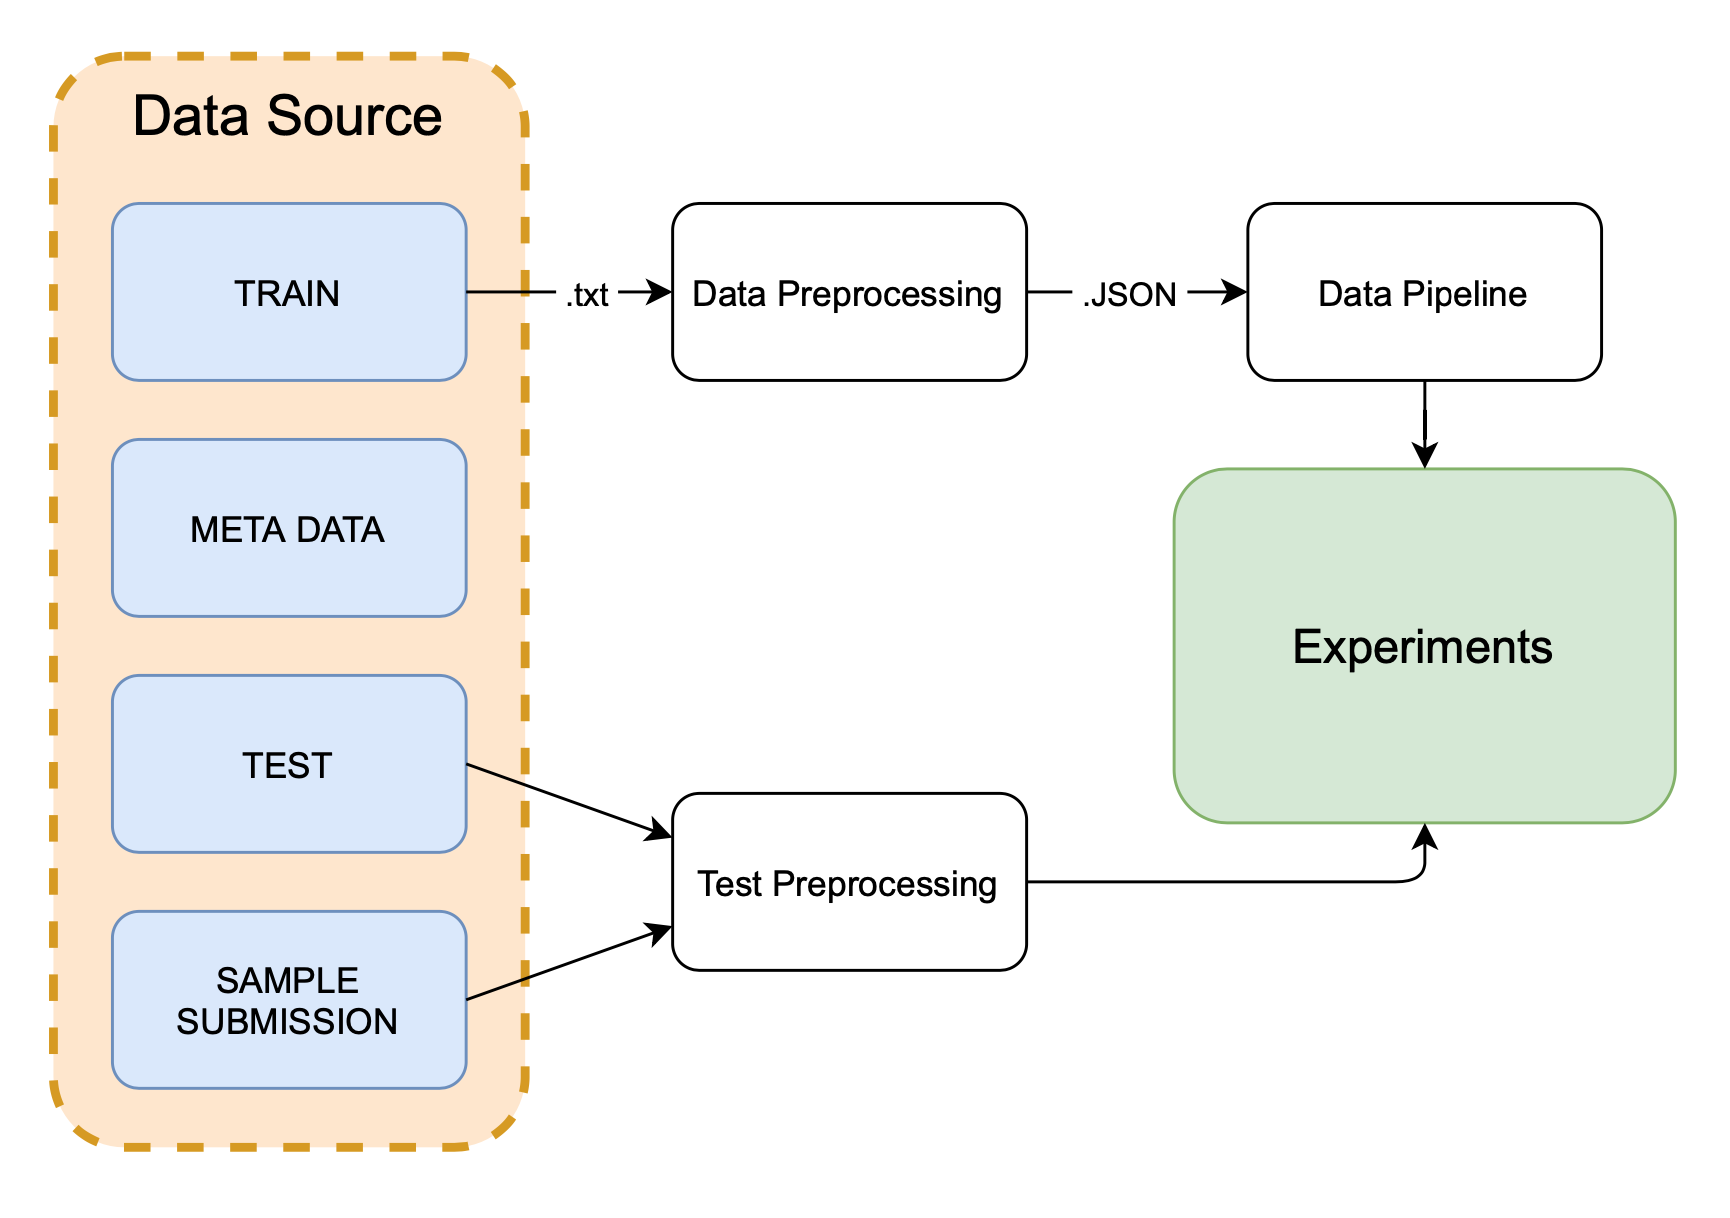
\includegraphics[scale=0.35]{Images/DataStandard/DataFlow.png}
    \caption{The overall architecture of data processing components}
    \label{fig:DataArchitecture}
\end{figure}

To determine how to prepare the data for scene analysis, we created an overall architecture of the data processing, which can be viewed on \textbf{\autoref{fig:DataArchitecture}}. The three different components, namely \textit{Data Preprocessing}, \textit{Data Pipeline} and \textit{Test Preprocessing} will be described in the following sections. The \textit{Data Preprocessing} will be divided into two parts: \textit{Train Data Conversion} and \textit{Train Data Cleaning}.

\subsection{Frameworks and Libraries}
%Python, pandas etc

\subsection{Train Data Conversion}
This process is a part of the \textit{Data Preprocessing} component depicted on \textbf{\autoref{fig:DataArchitecture}}. The first folder in the data source is the \textit{TRAIN} folder, which contains files on the regular text format, which we want to convert to \gls{json} format. The reason for this conversion is that \gls{json} is a universal data object format, supported by most languages by default or by adding a library. Additionally, we have chosen to remove the file structure, which first partitions the data into site and then floor level to instead simply add this information within each new \gls{json} file. This would result in \gls{json} files with a similar structure to \textbf{\autoref{fig:jsonformat}}.

\begin{figure}[H]
\lstset{numbers=left}
\begin{lstlisting}
{ 
    siteID:
    siteName:
    floorLevel:
    pathID:
    startTime:
    sensorData: 
        [
            {
                attributesFromKaggle
                label { x, y } // closest waypoint
            },
            {
                attributesFromKaggle
                label { x, y } // closest waypoint
            },
            ...
        ]
}
\end{lstlisting}
\caption{The \gls{json} format we have converted the data into.}
\label{fig:jsonformat}
\end{figure}

As seen on \textbf{\autoref{fig:jsonformat}}, each file contains information about which site (ID and name) and floor level the specific path has been measured at, alongside the ID of the path and a timestamp of when the measurement has begun. Lastly is an array containing the different sensor observations from the original path file. Each observation contains the original attributes, and we have determined and added the closest waypoint to each observation. The closest waypoint is determined by the timestamps meaning that the x- and y-coordinates for a sensor measurement are determined by the waypoint which is closest to the measurement. 

\subsection{Train Data Cleaning}
After processing the data to a new format, a level of data cleaning should also be enforced. This is concerned with normalising the floor level format to the same as the submission format. In the \gls{json} files the redundant data will be removed to minimise the size of each file. %Skal uddybes hvad er

%Problemet med new lines

%Outlier detection and removal such as looking whether the accelorometer values are proper.


\subsection{Data Pipeline} \label{sec:datapipeline}
After preprocessing, the data should be formatted after specific machine learning algorithms, which is depicted in \textbf{\autoref{fig:DataArchitecture}} as \textit{Data Pipeline}.

\subsection{Test Data Preprocessing}
\section{Data pipeline}
In this section, we will elaborate on the data pipeline for the experiments. The idea behind data pipeline is to automate the workflow for training and testing a model. 

\chapter{Experiments}
After processing the data, it is now possible to create different experiments for predicting locations. Before starting on the different experiments, we wanted to create a general pattern and flow of the experiments, which will be covered first. Thereafter, the different experiments and their evaluation will be covered.

\section{Experiment Flow}
To start off the process, we wanted to create an overall architecture similar to the one shown in \textbf{\autoref{fig:DataArchitecture}}. The data is being prepared for each individual experiment in the \textit{Data Pipeline} phase before reaching the \textit{Experiments} phase.

\begin{figure}[H]
    \centering
    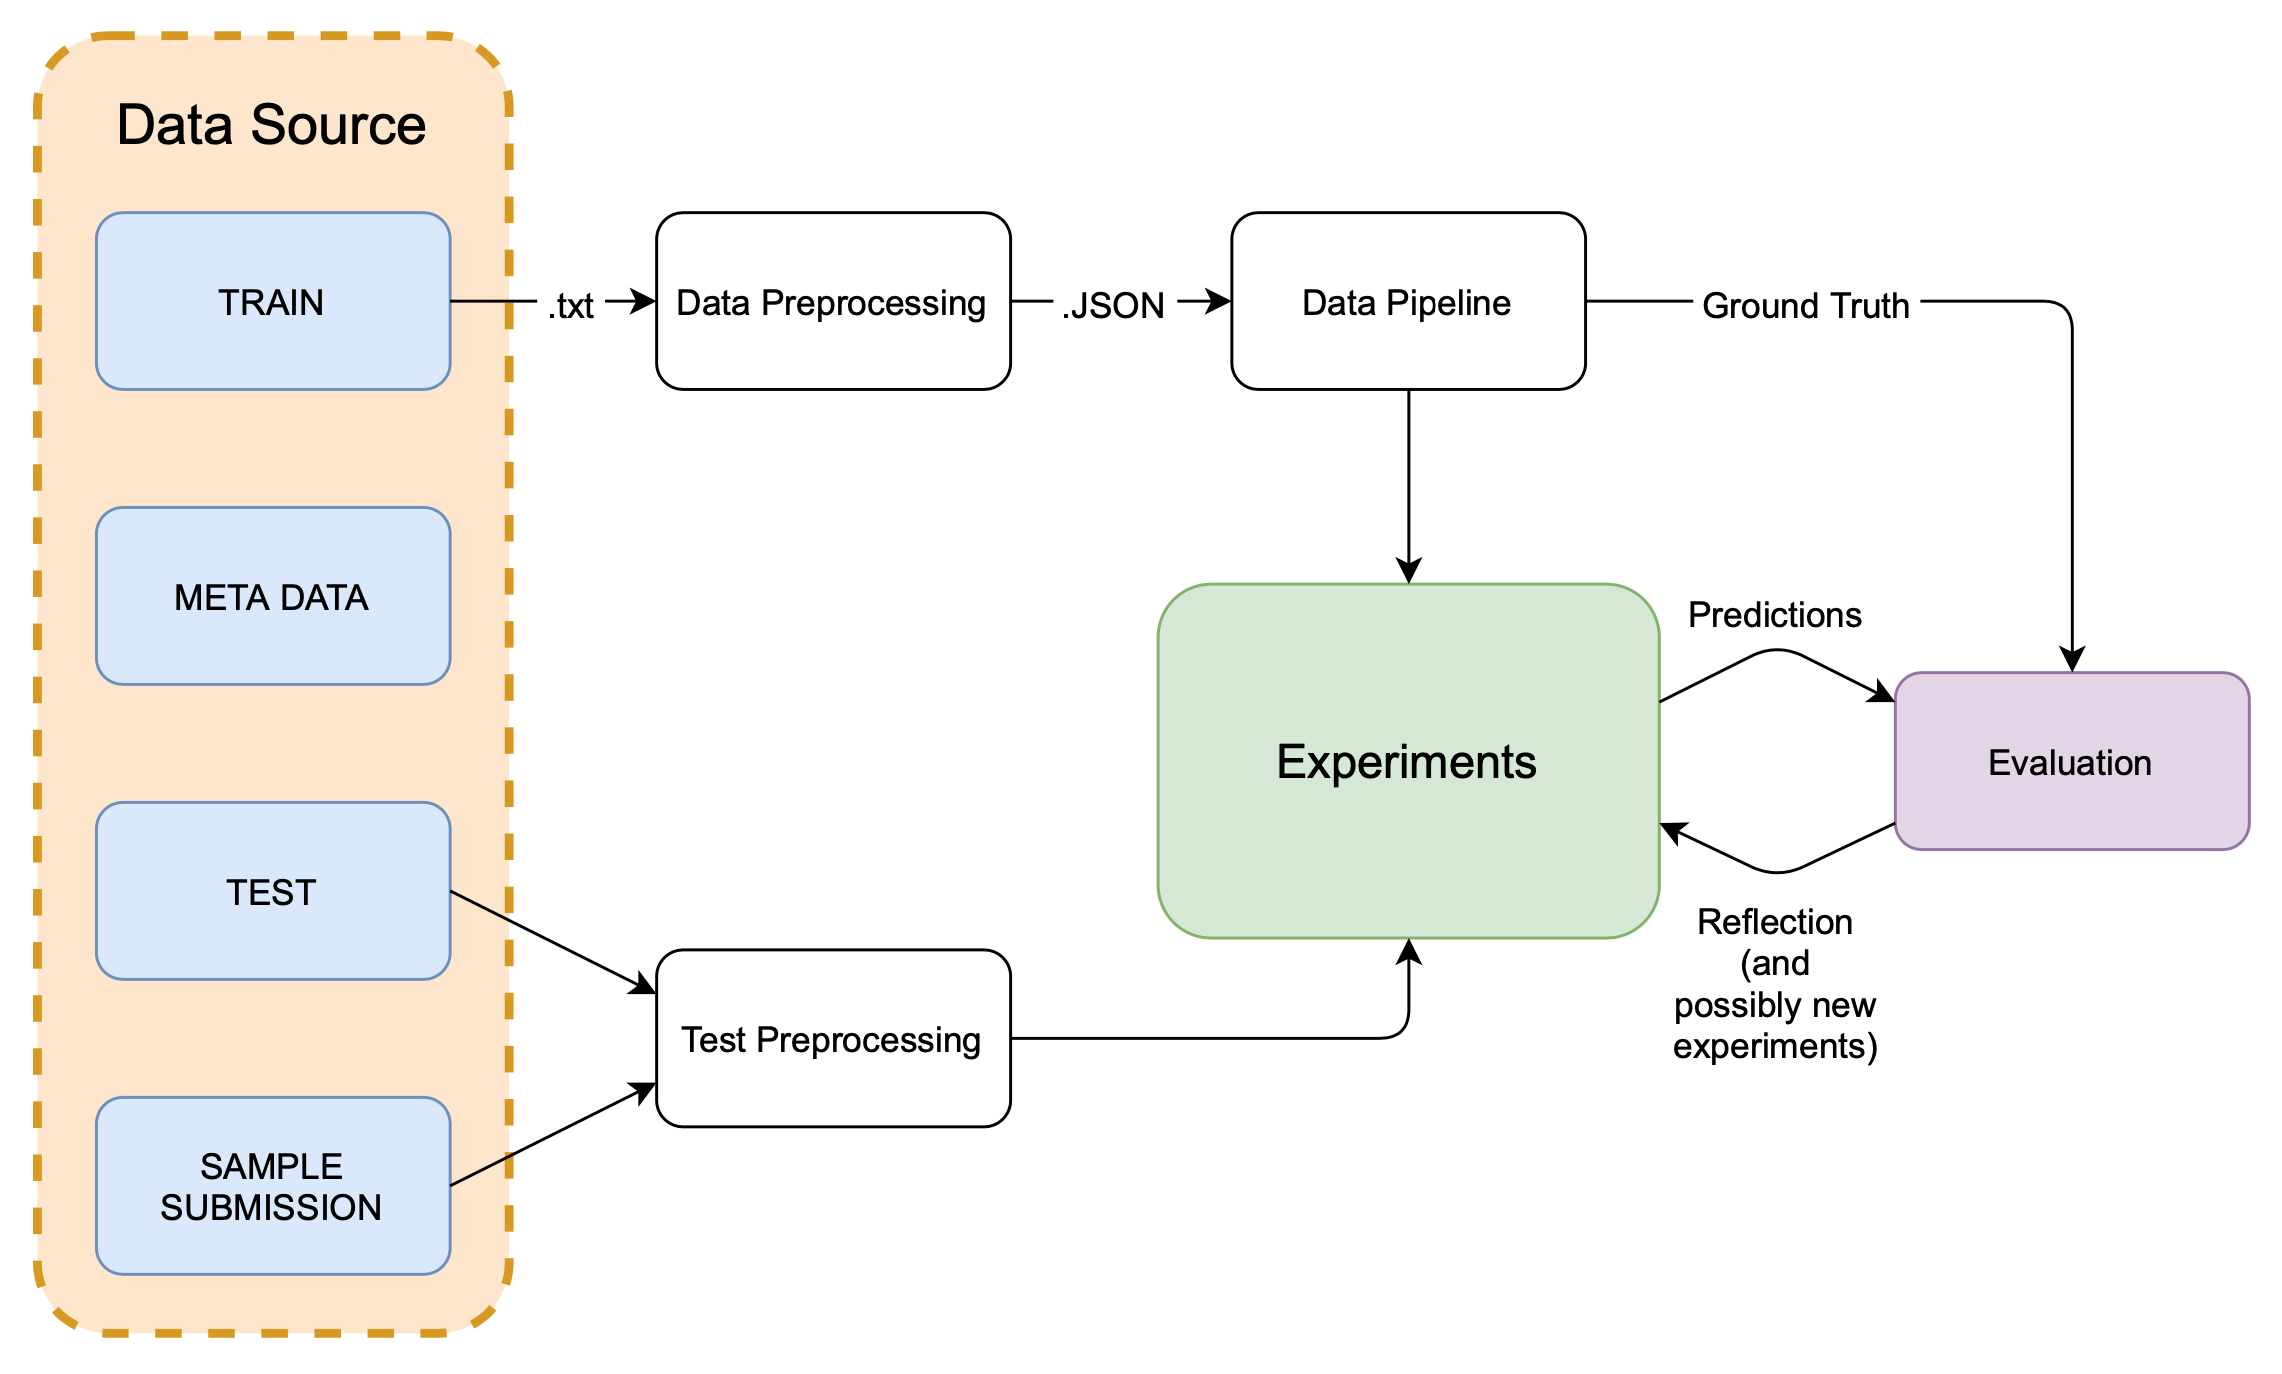
\includegraphics[scale=.34]{Images/Experiments/ExperimentFlow.png}
    \caption{The overall architecture with added evaluation.}
    \label{fig:experimentflow}
\end{figure}

As can be seen on \textbf{\autoref{fig:experimentflow}}, we have expanded on the \textit{Experiments} phase to also interact with the \textit{Evaluation} phase. This new phase takes the ground truth data and compares it to predictions from the experiment. For this purpose, the \textit{Data Pipeline} phase now passes the data to the Experiments phase and also the ground truth data for the \textit{Evaluation} phase. The \textit{Evaluation} phase now compares the result of the experiment to the ground truth and thereby evaluates the experiment. These results can be reflected on, which might lead to new experiments.

\subsection{Experiments}
The \textit{Experiments} phase in \textbf{\autoref{fig:experimentflow}} denotes the implementation and use of the positioning methods, mentioned in \textbf{\autoref{sec:problemstatement}}, which we would need to test. The different experiments will include LightGBM, \gls{ann}, \gls{hmm}, k-NN and \gls{imu}-based methods. Each experiment takes the input data from the \textit{Data Pipeline} phase. As mentioned in \textbf{\autoref{sec:datapipeline}}, this phase is concerned with processing the data for the specific positioning method in the experiment. After receiving the data from the \textit{Data Pipeline} phase, the implementation of the experiment will be executed to achieve estimations of the indoor locations. The estimations from these experiments will then be forwarded to the \textit{Evaluation} phase to determine the performance of the model.
%Elaborate the Experiment part of the design
%Generelt om hvad et eksperiment er + hvilke eksperimenter vi prøver af
%Kontekst til de andre dele (data pipeline + evaluation)
%Input og output til experiments
%

\subsection{K Fold Cross Validation}

\subsection{Evaluation}
To evaluate the different experiments, which is depicted as the \textit{Evaluation} component in \textbf{\autoref{fig:experimentflow}}, we have decided to model a generic Evaluator, which is responsible for the evaluation of the model/algorithm in term of different performance metrics.
%can be used within the experiment to evaluate the performance of the model. 
This Evaluator should evaluate the result with regards to the \gls{mpe} similar to the Kaggle competition mentioned in section \textbf{\autoref{sec:kaggleComp}}. Additionally, it should also calculate the position error with regards to each prediction made by the algorithm/model.

The Evaluator takes the estimations from the \textit{Experiments} phase and the ground truth data from the \textit{Data Pipeline} component as input. From this, it is possible to calculate the position error for each individual estimation. All of the performance metrics as well as the input to the Evaluator should be recorded to a files dedicated for evaluation output. The execution of the generic evaluation class should be integrated into each experiment, where it is possible to work with the results and maybe add additional evaluations.

% NOTER: 
% - Eksperimenter evalueres af single, central evaluator.
% Evaluate waypoints individually with position error
% Evaluator outputter resultater for hver enkelt waypoint.
%   Output indeholder ground truth, estimering, og position error for hvert enkelt prediction.
%   Output konkluderer med mean position error.
% Evaluatator tager ground truth data og estimeringer som input og udregner de nødvendige evalueringer og skriver dem i sidste ende til filer.
% Eksekvering af evaluator skal ske som en integreret del af hvert enkelt eksperiment.
% Evaluator skal generere output i 'output' folder.

%\subsection{Frameworks and Libraries}
%For implementing the different experiments and the generic evaluation class, we have decided to use the programming language Python for consistency with the development of the data handling. We also examined the possibility of implementing all these experiments, where Python seemed like an ideal programming language for this.

%To implement these experiments, we'll be using different frameworks and libraries. For some of the experiments, we have decided to use TensorFlow, which is an open-source machine learning platform.\cite{TensorFlow}
% Vi bruger Python til det hele udover til wrapper til libs.
% Vi bruger det der C++ library (https://github.com/derekblair/DeadReckoner)
% TensorFlow (Neural network, HMM, knn og RNN)
% LightGBM


%\subsection{Coding Standard}
% - Kommentar på alle metoder/funktioner/procedurer.
%   - Kommentarer skal komme den sidste linje før deklaration.
% - Snake-case til symbol deklarationer.
% - 
\section{Pedestrian Dead Reckoning}




The \gls{pdr} method is described in \cite{HybridPositioningPaper}. \gls{pdr} tracking is based on step detection algorithms, step length estimations $l_t$ and heading measurements $\theta_t$, all used to solve the problem defined in \textbf{\autoref{eq:pdr_x}} and \textbf{\autoref{eq:pdr_y}}.

\begin{equation} \label{eq:pdr_x}
    x_t = x_{t - 1} + l_t\cos(\theta_t)
\end{equation}

\begin{equation} \label{eq:pdr_y}
    y_t = y_{t - 1} + l_t\sin(\theta_t)
\end{equation}

\begin{figure}[H] \label{fig:pdr}
    \centering
    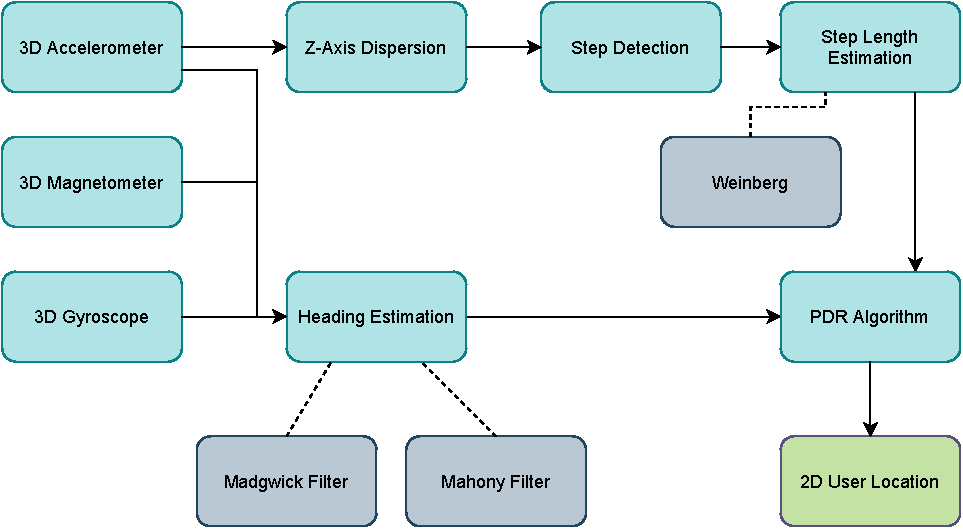
\includegraphics[scale=0.9]{Images/Experiments/pdr.pdf}
    \caption{PDR implementation architecture.}
\end{figure}

% Tag elementer fra filen geometry_based.tex fra 1.Problem_analysis til forklaring af PDR.

%https://link.springer.com/article/10.1186/1687-6180-2014-65

%Fast AHRS Filter for Accelerometer, Magnetometer,and Gyroscope Combination with Separated Sensor Corrections

%https://www.researchgate.net/profile/Pasquale-Cirillo-3/publication/303738116_A_comparison_of_multisensor_attitude_estimation_algorithms/links/5750181208aeb753e7b4a0c0/A-comparison-of-multisensor-attitude-estimation-algorithms.pdf

%http://www.cs.ndsu.nodak.edu/~siludwig/Publish/papers/SPIE20181.pdf

%https://core.ac.uk/download/pdf/31017028.pdf

\subsection{Step Detection}

The general idea of step detection of a pedestrian with a smartphone is by measuring the accelerometer sensor, and observe the increases and decreases in the acceleration pattern\cite{HybridPositioningPaper}. We have chosen to follow the algorithm proposed in \cite{peakdetection}. 

The algorithm is based on the principle of dispersion, which is the extent to which a distribution is stretched or squeezed. %https://en.wikipedia.org/wiki/Statistical_dispersion#cite_note-1

In this case, the algorithm will return a signal value if a new datapoint is a specific amount of deviations away from a moving mean. This amount of deviations is also called the z-score. The algorithm creates a separate moving mean and deviation, and signals can therefore not corrupt the threshold. The algorithm takes 3 inputs: lag, threshold and influence. Lag determines how much the input data is to be smoothened. Therefore, low lag values result in the algorithm being quicker at adapting to the input data. Since the input data for step detection vary a lot, the lag value will be low. The threshold is the z-score at which the algorithm will return a signal. Lastly, the influence is the impact of new signals on the mean and deviation. The influence can be between 0 and 1. If 0 is chosen as the influence, signals would be completely ignored for recalculation of a new threshold. This choice would assume stationarity, meaning that the statistical properties of a process, such as the mean, variance and the structure of the autocorrelation, do not change over time. In our case, we are working with data from walking people in a shopping mall, and since random walking is not a stationary process, we will use 1 as our influence. 

+ lag 
+ threshold


%https://stats.stackexchange.com/questions/246357/why-is-a-random-walk-not-a-stationary-process

%https://www.itl.nist.gov/div898/handbook/pmc/section4/pmc442.htm


%

%https://stackoverflow.com/questions/22583391/peak-signal-detection-in-realtime-timeseries-data/22640362

\subsection{Step Length Estimation}

For step length estimation, there exists two methods: static and dynamic. The static method assumes a person is walking at a constant velocity, whereas the dynamic method makes use of an accelerator for dynamic estimation. Weinberg is one method for dynamic step length estimation, and we have chosen to use the Weinberg method because of its low error compared to other methods \cite{HybridPositioningPaper}.

The Weinberg method is defined as in \textbf{\autoref{eq:weinberg}} \cite{weinberg}.

\begin{equation} \label{eq:weinberg}
    l = k \sqrt[4]{a_{LPF, peak} - a_{LPF, valley}}
\end{equation}

In \textbf{\autoref{eq:weinberg}}, $k$ is a constant factor, for example, $0.5$, $a_{LPF, peak}$ is the maximum acceleration in the z-axis and $a_{LPF, valley}$ is the minimum acceleration. 

\subsection{Heading Estimation}
Heading estimation is accomplished using \gls{ahrs}. \gls{ahrs} is a Python toolkit for estimation attitude containing several functions and utilities for the attitude estimation\cite{ahrs} and \cite{FastAHRS}. According to \cite{MultisensorComparison}, Madgwick and Mahony perform best in comparison to other alternative algorithms, both of which are provided by \gls{ahrs}. Both algorithms compute a set of quaternions, described in \textbf{\autoref{sec:quaternion}}, given a set of acceleration data and gyroscope data, from which a heading can be computed.

\subsection{Quaternions} \label{sec:quaternion}

\chapter{Technology}
\section{Mobility}
As the project which we are working with is an indoor positioning system and the motivation behind the project is to estimate and track the location of user based on data from a smartphone, we also need to look at the concept mobility, which is the overall theme of this project module. This is the case as the developed solution should be mobile. We will expand on the definition of mobility, approaches for building mobile applications/services, constraints for mobile applications/services. 

\subsection{Definition of Mobility}
Mobility is defined as the ability to move and are application or service that can be used when on the move on devices like smart phones, laptops and etc. When dealing with mobile application, the architecture types for mobile applications can broadly be divided into four, namely standalone, client-server, peer-to-peer, and hybrid. A standalone application means that no external communication is necessary for the application or service to function. In the client-server based application or service, the mobile application (client) will communicate to a third party through the HTTP protocol or an equivalent protocol. The peer-to-peer mobile systems make data communication possible by short range wireless communication (E.g. Bluetooth). The hybrid type support data communication by automatically switching between the client-server and peer-to-peer.

\subsection{Location Based Services}



\chapter{Design}

\chapter{Implementation}

\chapter{Evaluation}

\newpage
\listoftodos
\newpage

\renewcommand{\glsgroupskip}{}
\printglossaries

\addcontentsline{toc}{chapter}{References}

\printbibliography

\part{Appendix}
\appendix

%\markdownInput{offline.md}

%\part{Appendices}
%\appendixpageoff
%\begin{appendices}

%\end{appendices}
\end{document}